
\documentclass[calculator,steamtables,refrigeranttables,psychrometricchart,datasheet,solutions]{exam}
%\documentclass[calculator,steamtables,refrigeranttables,psychrometricchart,datasheet]{exam}

% The full list of class options are
% calculator : Allows approved calculator use.
% datasheet : Adds a note that data sheet are attached to the exam.
% handbook : Allows the use of the engineering handbook.
% resit : Adds the resit markings to the paper.
% sample : Adds conspicuous SAMPLE markings to the paper
% solutions : Uses the contents of \solution commands (and \solmarks) to generate a solution file

\usepackage{pdfpages}
\usepackage{lscape,comment}

\coursecode{EG3521}%%
\coursetitle{Engineering Thermodynamics}%
%\coursecode{EG3539}% 
%\coursetitle{Thermodynamics}%

\examtime{00.00--00.00}%
\examdate{00}{05}{2015}%
\examformat{Candidates must attempt \textit{all} questions.}

\newcommand{\frc}{\displaystyle\frac}
\newcommand{\br}[1]{\!\left( #1 \right)}
\newcommand{\abs}[1]{\left| #1 \right|}
\newcommand{\fracd}[2]{\frac{\mathrm{d} #1}{\mathrm{d} #2}}
\newcommand{\fracp}[2]{\frac{\partial #1}{\partial #2}}
\renewcommand{\d}[1]{\mathrm{d} #1 }
\newcommand{\Ma}{\mathrm{M\!a}}



\begin{document}

%%%
%%% QUESTION 1
%%%
\begin{question}

\begin{enumerate}[(i)]

%%%  Q(1.i) Diesel: Example 13.22 (Rajput)
\item The volume ratios of compression and expansion for a diesel engine are 15.3 and 7.5, respectively. The pressure and temperature at the beginning of the compression are 1 bar and 27 $^{\text{ o}}$C. Assume that the volume at the end of the isentropic compression is 1 m$^{3}$, determine:
\begin{enumerate}[(a)]
 \item Mean effective pressure $\left(\text{MEP}=\frc{\text{W}_{\text{net}}}{\text{V}_{\text{max}}-\text{V}_{\text{min}}}\right)$;~\marks{7}
%
\solution{ The problem gives: 
     \begin{center}
      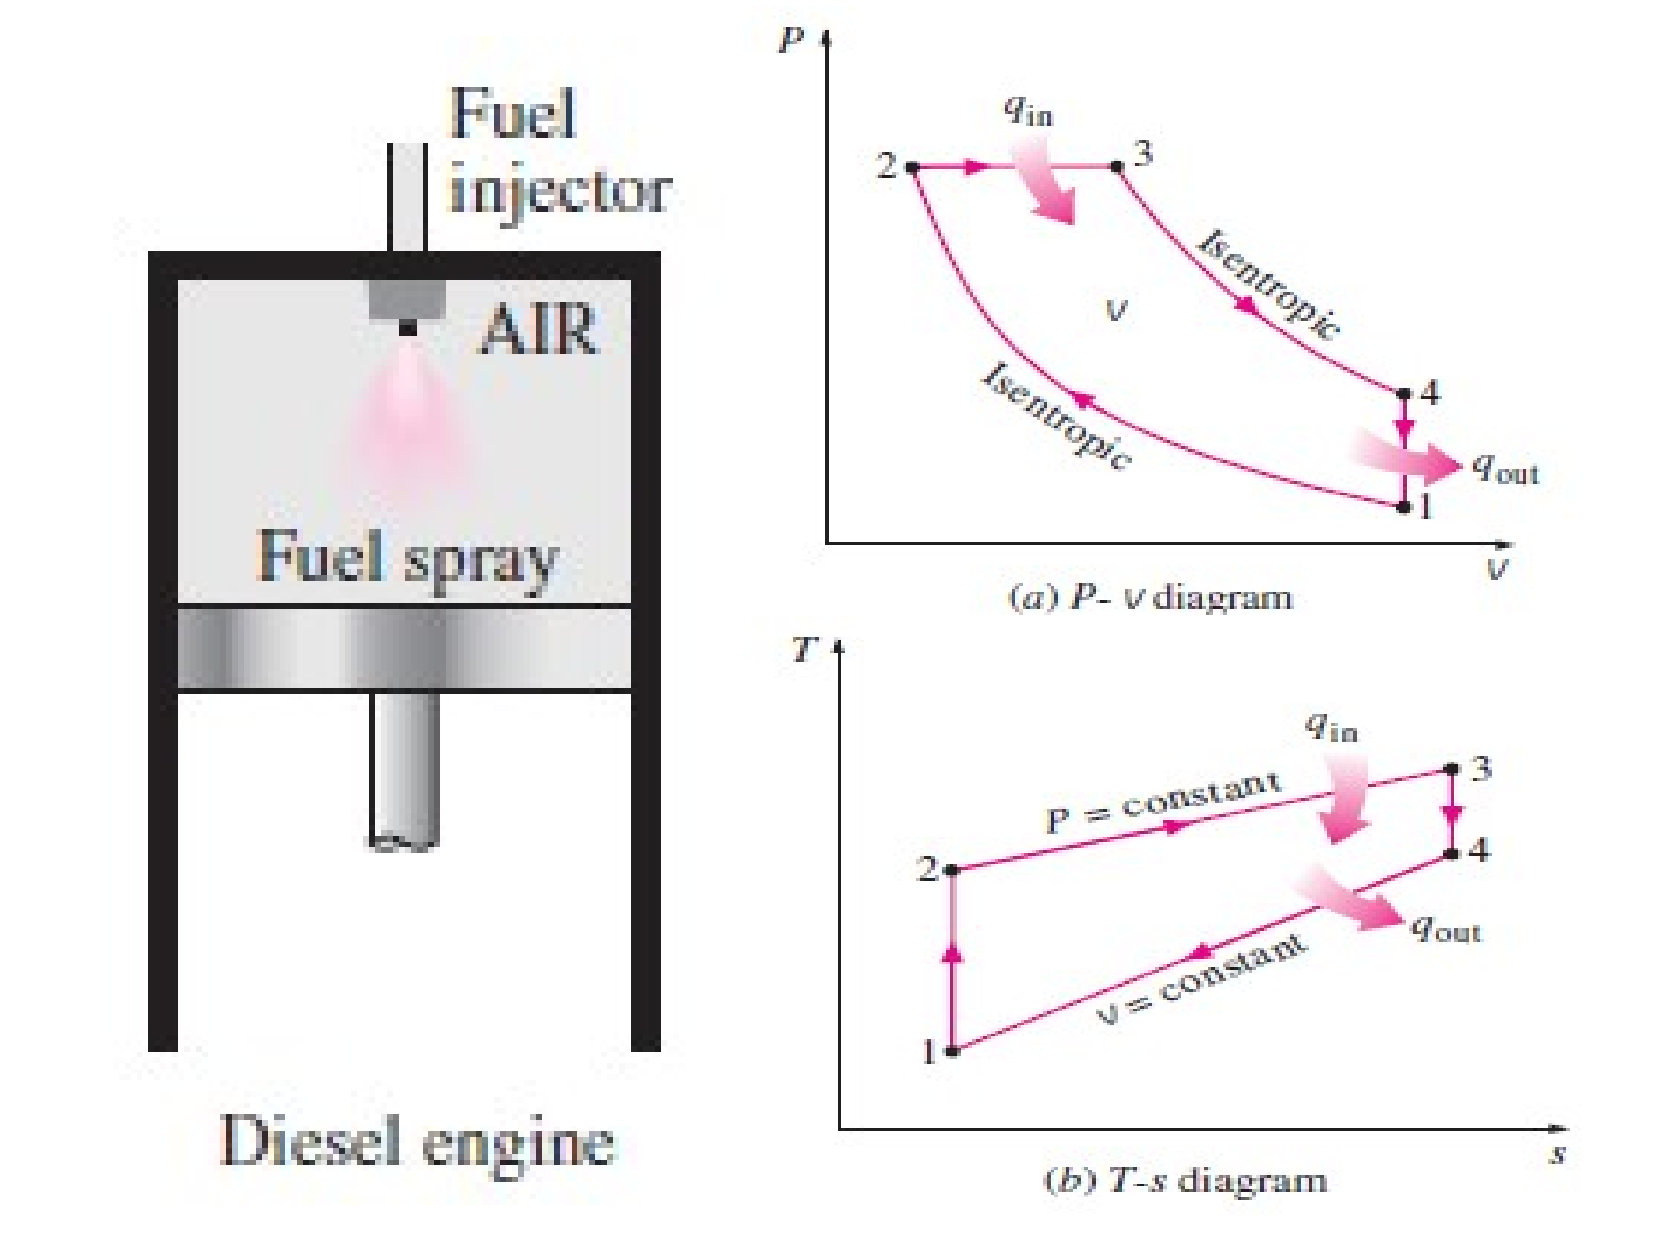
\includegraphics[width=6.cm,clip]{../Thermodynamics/EngThermod/2014-15/Lectures/Pics/InternalCombustion_IdealDieselCycle}
     \end{center} 
\begin{itemize}
 \item $\frc{V_{1}}{V_{2}}$ = 15.3 = r, $\frc{V_{4}}{V_{3}}$ = 7.5;
 \item $P_{1}$ = 1 bar; $T_{1}$ = 27$^{\circ}$C = 300.15 K; V$_{2}$ = 1 m$^{3}$
\end{itemize}


The first step to solve the problem is to calculate T$_{2}$, P$_{2}$, T$_{3}$, T$_{4}$ and P$_{4}$:
\begin{description}
\item[1-2:] adiabatic compression:  ~\solmarks{1/7} 
\begin{eqnarray}
&& T_{1}V_{1}^{\gamma-1}=T_{2}V_{2}^{\gamma-1} \rightarrow T_{2} = 893.75\; \text{K} \nonumber  \\
&& P_{1}V_{1}^{\gamma}=P_{2}V_{2}^{\gamma} \rightarrow P_{2} = 45.56\; \text{bar}  \nonumber
\end{eqnarray}

\item[2-3:] heat addition at constant pressure: ~\solmarks{0.5/7}
\begin{displaymath}
\frc{V_{2}}{T_{2}} = \frc{V_{3}}{T_{3}} \rightarrow T_{3} = T_{2}\frc{V_{3}}{V_{1}}\frc{V_{1}}{V_{2}} = 1823.25\text{ K }
\end{displaymath}

\item[3-4:] adiabatic expansion:~\solmarks{1/7} 
\begin{eqnarray}
&& T_{3}V_{3}^{\gamma-1}=T_{4}V_{4}^{\gamma-1} \rightarrow T_{4} = 814.37\; \text{K} \nonumber  \\
&& P_{3}V_{3}^{\gamma}=P_{4}V_{4}^{\gamma} \rightarrow P_{4} = 2.71\; \text{bar}  \nonumber
\end{eqnarray}
\end{description}

Now calculating MEP:~\solmarks{1.5/7}
\begin{displaymath}
MEP = \frc{W_{\text{net}}}{V_{\text{max}}-V_{\text{min}}} = \frc{m\left[C_{p}\left(T_{3}-T_{2}\right) - C_{v}\left(T_{4}-T_{1}\right)\right]}{V_{1}-V_{2}}
\end{displaymath}
 now we need to calculate the mass (m) via the equation of state of ideal gas at state 2:~\solmarks{1/7}
\begin{displaymath}
m = \frc{P_{2}V_{2}}{R T_{2}} MW = 17780.98 g \approx 17.78\; kg
\end{displaymath}
with the mass of air, the MEP is 7.02 bar~\solmarks{2/7}
}
%
 \item Cycle efficiency $\left(\eta_{\text{Diesel}}=\frc{\text{W}_{\text{net}}}{\text{Heat Supplied}}\right)$;~\marks{3}
\solution{The efficiency of the Diesel engine is given by:~\solmarks{3/3}
\begin{displaymath}
\eta_{\text{Diesel}} = \frc{W_{\text{net}}}{\text{Heat Supplied}} = \frc{m\left[C_{p}\left(T_{3}-T_{2}\right) - C_{v}\left(T_{4}-T_{1}\right)\right]}{m C_{p}\left(T_{3}-T_{2}\right)} = 0.6048
\end{displaymath}
}
%
\end{enumerate}

%%% Q(1.ii) Brayton: Example 10.1 (Borgnakke )
\item In an air-standard Brayton cycle, the air enters the compressor at 0.1 MPa and 15$^{\circ}$C. The pressure leaving the compressor is 1 MPa and the maximum temperature in the cycle is 1100$^{\circ}$C. Determine:
\begin{enumerate}
\item Sketch the schematics and the thermodynamic diagrams ($Pv$ and $Ts$) of the cycle, numbering each stage;~\marks{2}
\solution{ Schematics, $Pv$ and $Ts$ diagrams:\solmarks{2/2}
   \begin{center}%
     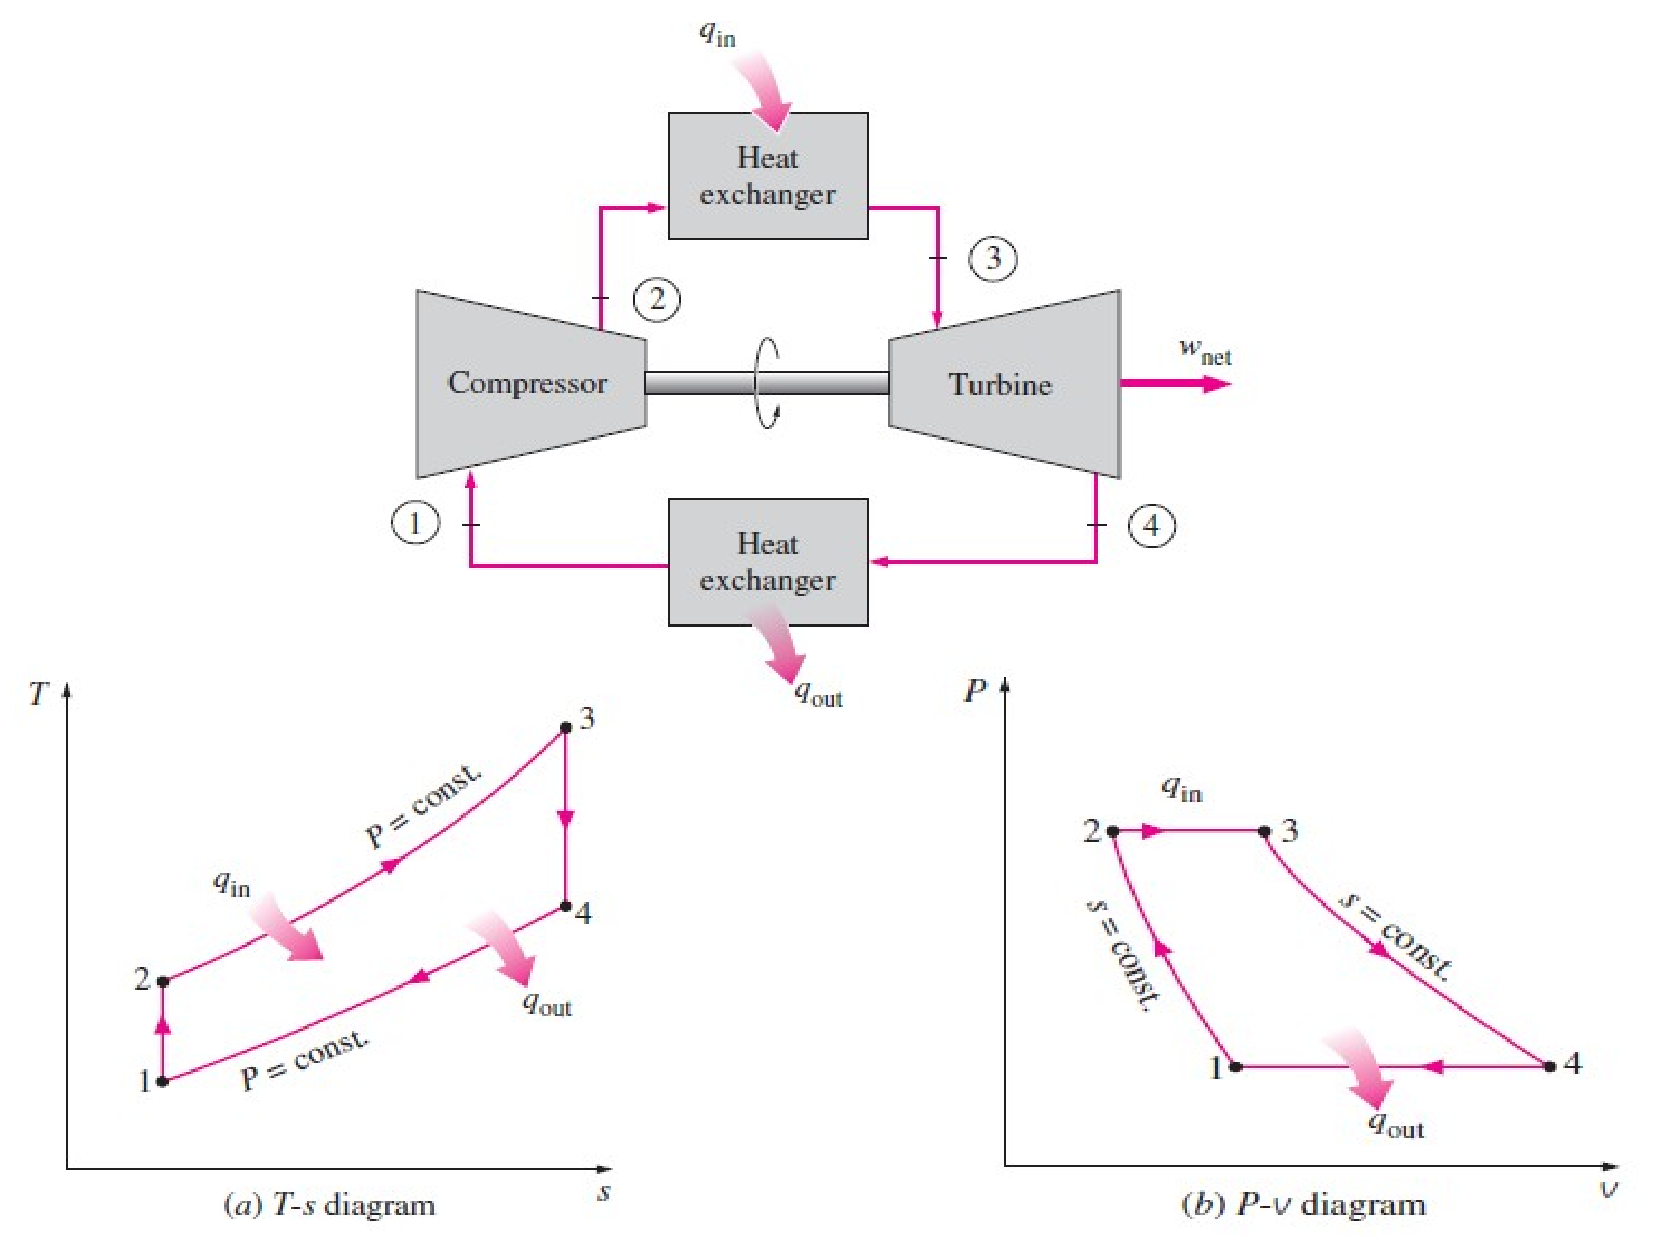
\includegraphics[height=8.cm,width=8.5cm,clip]{../Thermodynamics/EngThermod/2014-15/Lectures/Pics/Brayton_cycle1}
   \end{center}  
}
%
\item Temperatures of the fluid leaving the compressor and turbine;~\marks{2}
\solution{ Calculating T$_{2}$ and T$_{4}$:
\begin{description}
\item[1-2:] isentropic compression: \solmarks{1/2}
\begin{displaymath}
T_{1}P_{1}^{\frac{1-\gamma}{\gamma}} = T_{2}P_{2}^{\frac{1-\gamma}{\gamma}} \rightarrow T_{2} = 556.33\text{ K}
\end{displaymath}
\item[3-4:] isentropic expansion: \solmarks{1/2}
\begin{displaymath}
T_{3}P_{3}^{\frac{1-\gamma}{\gamma}} = T_{4}P_{4}^{\frac{1-\gamma}{\gamma}} \rightarrow T_{4} = 711.22 \text{ K}
\end{displaymath}
\end{description}
}
%
\item Efficiency of the cycle $\left(\eta_{\text{Brayton}}=\frc{\text{W}_{\text{net}}}{\text{Heat Supplied}}\right)$;~\marks{2}
\solution{ Work required by the compressor~\solmarks{0.5/2} 
\begin{displaymath}
W_{\text{C}} = h_{2}-h_{1} = C_{p}\left(T_{2}-T_{1}\right) = 269.52 \text{ kJ.kg}^{-1}
\end{displaymath}
And the work produced by the turbine:~\solmarks{0.5/2}
\begin{displaymath}
W_{\text{T}} = h_{4}-h_{3} = C_{p}\left(T_{4}-T_{3}\right) = -665.24 \text{ kJ.kg}^{-1}
\end{displaymath}
The efficiency is given by:~\solmarks{1/2}
\begin{displaymath}
\eta_{\text{Brayton}} = \frc{W_{\text{net}}}{\text{heat supplied}} = \frc{\left|W_{T}+W_{C}\right|}{C_{p}\left(T_{3}-T_{2}\right)} = 0.4821
\end{displaymath}
}
%
\item Assume that the efficiency of the compressor and the turbine are 80$\%$ and 85$\%$, respectively, and the pressure drop between the compressor and the turbine is 15 kPa. Calculate the work in the compressor and turbine, and the efficiency of the cycle.~\marks{4}
\end{enumerate}

\end{enumerate}
For this question, assume that air behaves as an ideal gas with the following properties: MW = 29 g.mol$^{-1}$, C$_{p}$ = 1.005 kJ.(kg.K)$^{-1}$ and C$_{v}$ = 0.718 kJ.(kg.K)$^{-1}$, where MW is the molar mass and C$_{p}$ and C$_{v}$ are the heat capacities at constant pressure and volume, respectively. Also, given the following relations with $\gamma \equiv \displaystyle\frac{C_{P}}{C_{V}}$
\begin{displaymath}
TV^{\gamma-1}=\text{const.} \Leftrightarrow TP^{\frac{1-\gamma}{\gamma}}=\text{const.} \Leftrightarrow PV^{\gamma}=\text{const.} 
\end{displaymath}


\end{question}








%%%
%%% Question 01 
%%%
\begin{question}
%
A geothermal power station (Rankine cycle) uses propane $\left(\text{n-C}_{3}\right)$ as working fluid to produce power $\left(W_{T}\right)$ in a turbine (isentropic expansion) with efficiency $\left(\eta_{T}\right)$ of 90$\%$. n-C$_{3}$ is vaporised by geothermal water (brine, $A-B$ in the diagram) at 90$^{\circ}$C. After condensed, n-C$_{3}$ is driven to a heat exchanger (with thermal efficiency of 68$\%$) and the cycle continues. The mass flow rate of n-C$_{3}$ $\left(\dot{m}_{C3}\right)$ is 250 kg.s$^{-1}$ and the heat capacity at constant pressure $\left(C_{p}\right)$ of brine is 3565.5 J.(kg.K)$^{-1}$. Conditions for n-C$_{3}$ and brine flows are described in Table below.
%\vspace{-.9cm}
\begin{center}
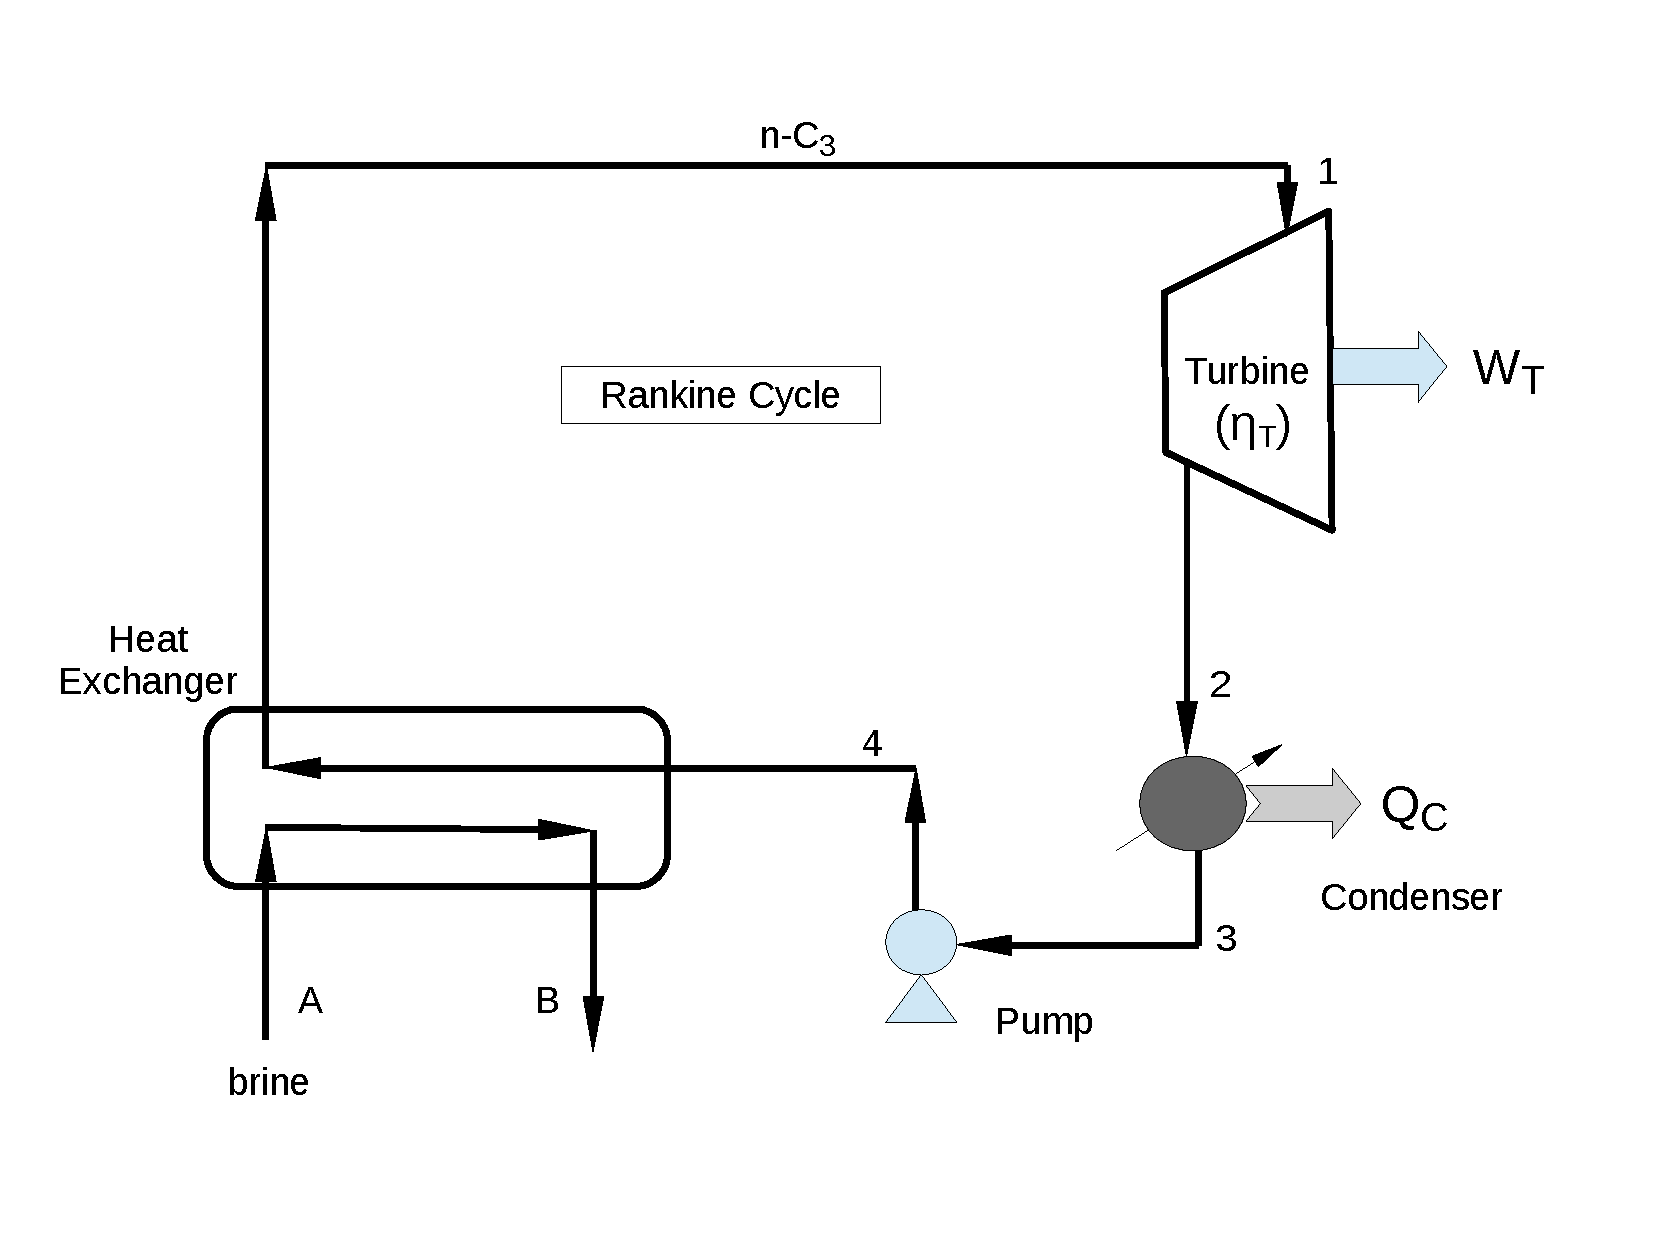
\includegraphics[width=10.cm,height=7.cm,clip]{./Pics/RankineCycle}
%\caption{ Reheat and regenerative Rankine cycle with 2 turbines.}
%\label{exam_mod02_rankinecycle}
\end{center}
%\vspace{-1.5cm}
\begin{center}
\begin{tabular} {||c | c c c c c || }
\hline\hline
{\bf Stage} & {\bf P}    & {\bf T}        & {\bf State}    & {\bf h}             & {\bf s}                  \\
            & {\bf (bar)}& {\bf ($^{o}$C)} &               & {\bf (kJ.kg$^{-1}$)} & {\bf (kJ.(kg.K)$^{-1}$)}  \\
\hline\hline
 {\bf 1 }   & 16         & 50             &   {\bf (a)}    & {\bf (b)}           & {\bf (c)}                \\
 {\bf 2 }   & 6          &  --            &   wet vapour   & {\bf (d)}           & --                       \\
 {\bf 3 }   & 6          &                &   sat. liquid  & {\bf (e)}           & --                       \\
 {\bf 4 }   & 16         &                &   {\bf (f)}    & {\bf (g)}           & --                       \\
 {\bf A }   & --         & 90             &   --           & --                  & --                       \\
 {\bf B }   & --         & 30             &   --           & --                  & --                       \\
 \hline\hline
\end{tabular}
\end{center}

\begin{enumerate}[(a)]
%%
%% Question A
%%
\item In this Table, determine {\it (a)-(g)}.~\marks{7}
%
\solution{
In order to fill the Table we need to calculate the thermodynamic properties for each stage of the cycle:
\begin{description}
%%%
\item[Stage 1:] At P$_{1}$ = 16 bar, T$_{1}$ = 50$^{\circ}$C $>$ T$_{sat}\left(P_{1}\right)$ = 46.89$^{\circ}$C. Therefore the fluid is at {\bf superheated state}~\solmarks{1/7}. From the superheated table for n-C$_{3}$ at P$_{1}$ and T$_{1}$, we can obtain:\\
{\bf H$_{1}$ = 522.5 kJ.kg$^{-1}$}~\solmarks{1/7} and\\
{\bf S$_{1}$ = 1.733 kJ.(kg.K)$^{-1}$}~\solmarks{1/7}. 
%%%
\item[Stage 2:] At P$_{2}$ = 6 bar, the fluid is wet vapour after the isentropic expansion. We should first calculate the quality of the vapour in an ideal expansion (using values of entropy/enthapy obtained from the saturated n-C$_{3}$ table at P$_{2}$.
\begin{displaymath}
x_{2s} =\frc{S_{2s}-S_{f}}{S_{g}-S_{f}} = \frc{1.733 - 0.446}{1.737-0.446} = 0.9969
\end{displaymath}
now to calculate the ideal enthalpy,
\begin{displaymath}
x_{2s} = 0.9969 = \frc{H_{2s}-H_{f}}{H_{g}-H_{f}} = \frc{H_{2s}-115.3}{478.3-115.3}\;\;\Longleftrightarrow\;\; H_{2s} = 477.17 \frc{kJ}{kg}
\end{displaymath}
As the efficiency of the turbine is of 90$\%$,
\begin{displaymath}
\eta_{\text{Turbine}} = 0.90 =\frc{H_{2}-H_{1}}{H_{2s}-H_{1}} = \frc{H_{2} - 522.5}{477.17 - 522.5} \;\;\Longleftrightarrow \;\; {\bf H_{2} = 481.70\frc{kJ}{kg}}
\end{displaymath}~\solmarks{1/7}
%%%
\item[Stage 3:] At P$_{3}$ = P$_{2}$ = 6 bar, the fluid leaving the condenser towards the pump is saturated liquid, and the enthalpy and specific volume are the same of the liquid phase obtained from the saturated table:\\
{\bf H$_{3}$} = H$_{f}\left(\text{P = 6 bar}\right)$ {\bf = 115.3 kJ.kg$^{-1}$}~\solmarks{1/7} \\
V$_{3}$ = V$_{f}\left(\text{P = 6 bar}\right)$ = 1.931$\times$10$^{-3}$ m$^{3}$.kg$^{-1}$ 
%%%
\item[Stage 4:] The fluid leaving the pump is {\bf sub-cooled liquid}.~\solmarks{1/7} As there is no heat loss in the pump, we can assume $dH \approx VdP$, therefore
\begin{displaymath}
{\bf H_{4}} = H_{3} + V_{3}\left(P_{4}-P_{3}\right) = 115.3\frc{kJ}{kg} + 1.931\times 10^{-3} \frc{m^{3}}{kg} \left(16 - 6\right)\text{bar} {\bf= 117.23 \frc{kJ}{kg}}
\end{displaymath}~\solmarks{1/7}

\end{description}
Thus the Table becomes:
\begin{center}
\begin{tabular} {||c | c c c c c || }
\hline\hline
{\bf Stage} & {\bf P}    & {\bf T}        & {\bf State}    & {\bf h}             & {\bf s}                  \\
            & {\bf (bar)}& {\bf ($^{o}$C)} &               & {\bf (kJ.kg$^{-1}$)} & {\bf (kJ.(kg.K)$^{-1}$)}  \\
\hline\hline
 {\bf 1 }   & 16         & 50             &{\bf superheated vapour}&{\bf 522.5}  & {\bf 1.733}              \\
 {\bf 2 }   & 6          &  --            &   wet vapour   & {\bf 481.70}        & --                       \\
 {\bf 3 }   & 6          &                &   sat. liquid  & {\bf 115.3}         & --                       \\
 {\bf 4 }   & 16         &                &{\bf sub-cooled liquid}& {\bf 117.23} & --                       \\
 {\bf A }   & --         & 90             &   --           & --                  & --                       \\
 {\bf B }   & --         & 30             &   --           & --                  & --                       \\
 \hline\hline
\end{tabular}
\end{center}
}
%%
%% Question B
%%
\item Calculate the power produced by the turbine $\left(W_{T}\right)$ and the heat extracted in the condenser $\left(Q_{C}\right)$ in {\it MW}.~\marks{2}
%
\solution{
\begin{displaymath}
{\bf W_{T}} = \dot{m}_{C3} \left(H_{1}-H_{2}\right) = 250\frc{kg}{s} \times \left(522.5 - 481.70\right)\frc{kJ}{kg} = 10200 \frc{kJ}{s} {\bf = 10.2 MW}
\end{displaymath}~\solmarks{1/2}

\begin{displaymath}
{\bf Q_{C}} = \dot{m}_{C3} \left(H_{2}-H_{3}\right) = 250\frc{kg}{s} \times \left(481.70 - 115.30\right)\frc{kJ}{kg} = 91600 \frc{kJ}{s} {\bf = 91.6 MW}
\end{displaymath}~\solmarks{1/2}
} 
%%
%% Question C
%%
\item Calculate the mass flow rate of brine in {\it kg.s}$^{-1}$.~\marks{3}
%
\solution{
The heat extracted by the n-C$_{3}$ $\left(\dot{Q}_{C3}\right)$ fluid in the heat exchanger can be easily calculated by
\begin{displaymath}
{\bf \dot{Q}_{C3}} = \dot{m}_{C3}\left(H_{1}-H_{4}\right) {\bf = 101317.5\frc{kJ}{s}}
\end{displaymath}~\solmarks{1/3}
Assuming that the heat extracted from the geothermal fluid (brine), $\dot{Q}_{gf}$ is transferred to the n-C$_{3}$ stream with efficiency of 68$\%$,
\begin{displaymath}
\eta_{\text{HE}} = 0.68 = \frc{\dot{Q}_{C3}}{\dot{Q_{gf}}} \;\; \Longleftrightarrow  {\bf \dot{Q}_{gf} = 148996.32 \frc{kJ}{s}}
\end{displaymath}~\solmarks{1/3}
With the heat generated by the geothermal fluid and the inlet/outlet fluid temperatures, we can now calculate the brine mass flow rate for the associated heat transferred,
\begin{displaymath} 
\dot{Q}_{gf} = 148996.32 \frc{kJ}{s} = \dot{m}_{gf} C_{p} \left(T_{A} - T_{B}\right)  \;\;\Longleftrightarrow\;\; {\bf \dot{m}_{gf} = 696.57\frc{kg}{s}}
\end{displaymath}~\solmarks{1/3}
}
%%%
%%% Question D
%%%
\item Sketch the temperature $\times$ entropy (TS) diagram for the process indicating the liquid and vapour saturated lines and each stage of the n-C$_{3}$ Rankine cycle.~\marks{3}
%
\solution{~\solmarks{3/3}
\begin{center}
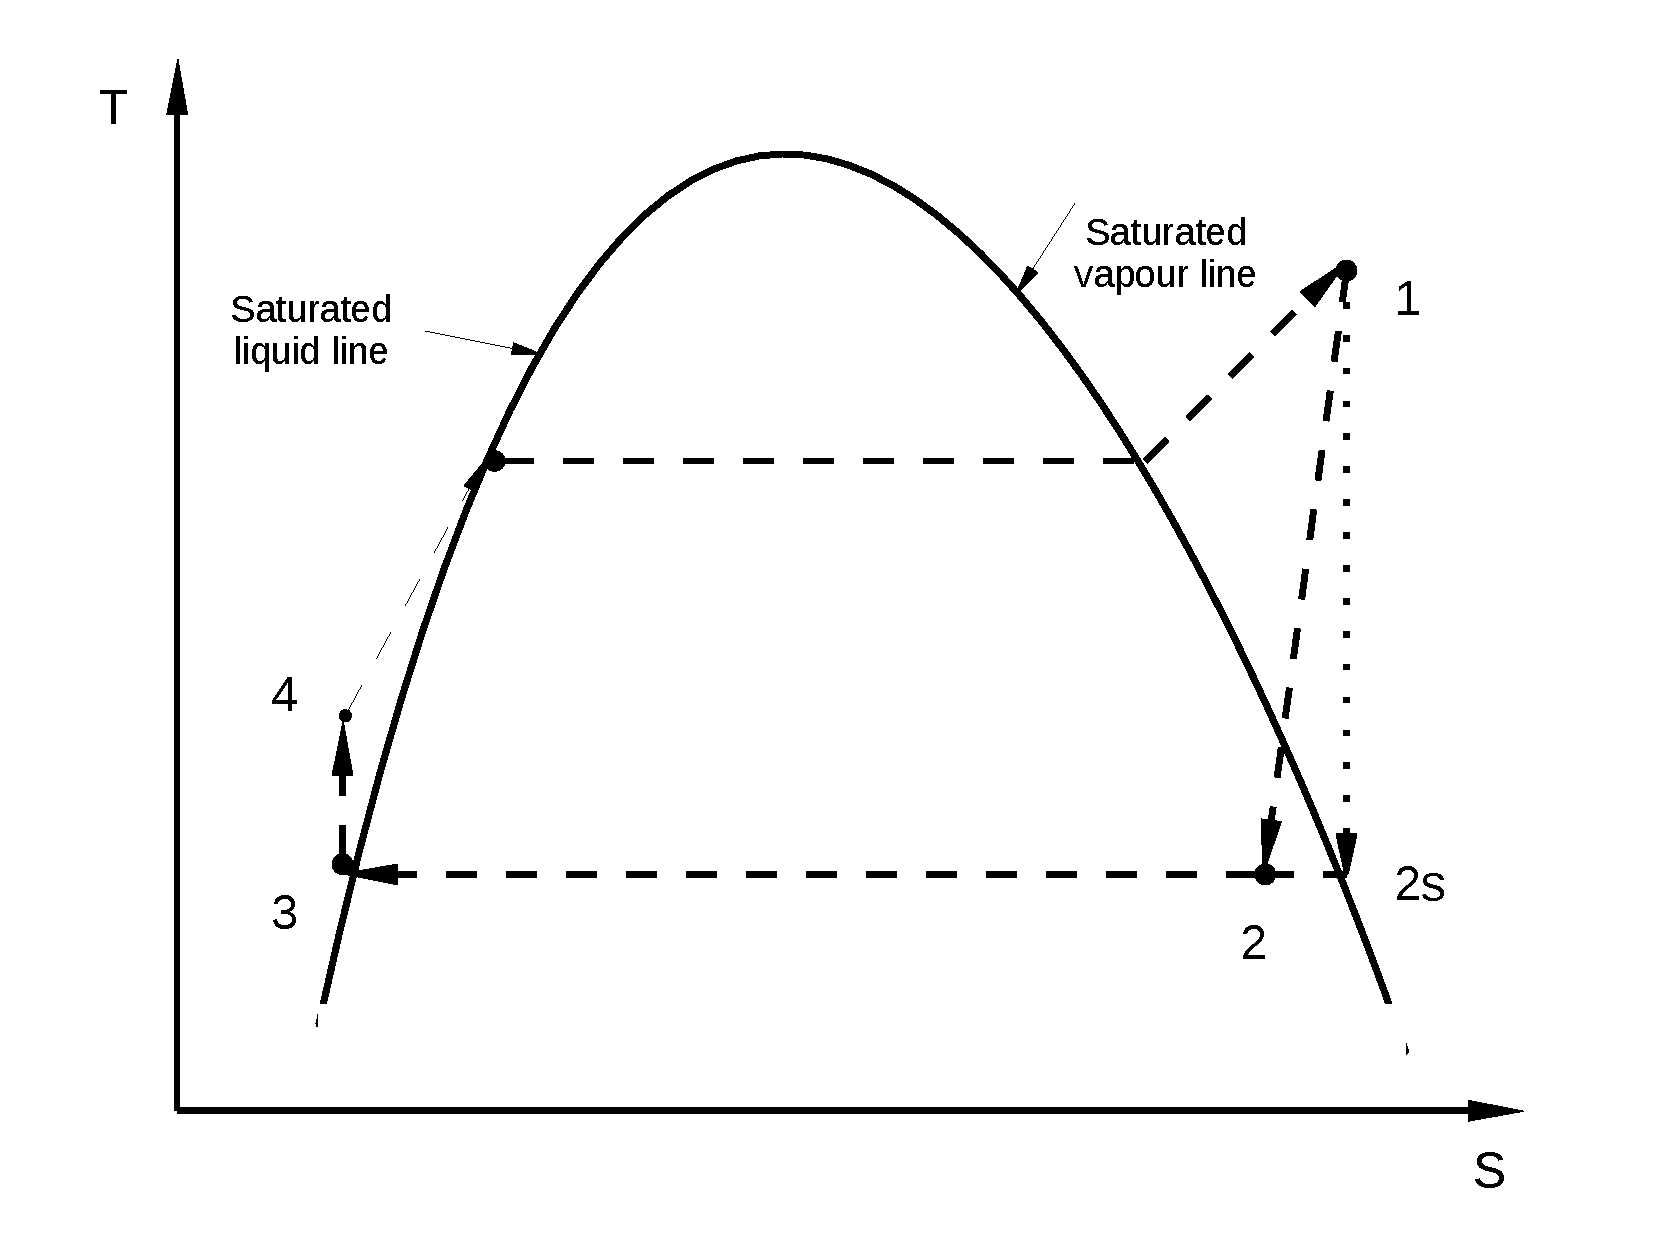
\includegraphics[width=8.cm,clip]{./Pics/TS_DIagramGeothermalBinary}
\end{center}%~\solmarks{3/3}
}
\end{enumerate} 

To solve this problem, you should assume that the saturated liquid streams are incompressible, and therefore $dH = VdP$ (where $H$, $V$ and $P$ are enthalpy, volume and pressure, respectively). Quality of the vapour is expressed as
\begin{displaymath}
x_{j} = \frc{\Psi_{j}-\Psi_{f}}{\Psi_{g}-\Psi_{f}}\;\;\;\text{with }\Psi=\left\{H,S\right\}
\end{displaymath}
where $S$ is the entropy. Efficiency of the turbine $\left(\eta_{\text{Turbine}}\right)$ and the heat exchanger $\left(\eta_{\text{HE}}\right)$ are given by,
\begin{displaymath}
\eta_{\text{Turbine}} =\frc{H_{2}-H_{1}}{H_{2s}-H_{1}} \;\;\;\text{ and }\;\;\; \eta_{\text{HE}} = \frc{\dot{Q}_{C3}}{\dot{Q_{gf}}}
\end{displaymath}
where $H_{2s}$ is the enthalpy of stream $2$ assuming ideal turbine performance (i.e., reversible expansion). $\dot{Q}_{C3}$ and $\dot{Q}_{gf}$ are the heat associated with the n-C$_{3}$ and brine streams, respectively, at the heat exchanger.

%
\end{question}





%%%
%%% Question 01 
%%%
\begin{question} %\vspace{-2\baselineskip}
A steam power plant operates with coupled regenerative and reheat Rankine cycle with 2 connected turbines as shown in Fig. \ref{exam_mod02_rankinecycle}.  Primary steam is supplied by the boiler at 120 bar and 565$^{\text{o}}$C. Conditions for water/steam flows are described in Table \ref{exam1_table1}. 

\begin{figure}[h]
\begin{center}
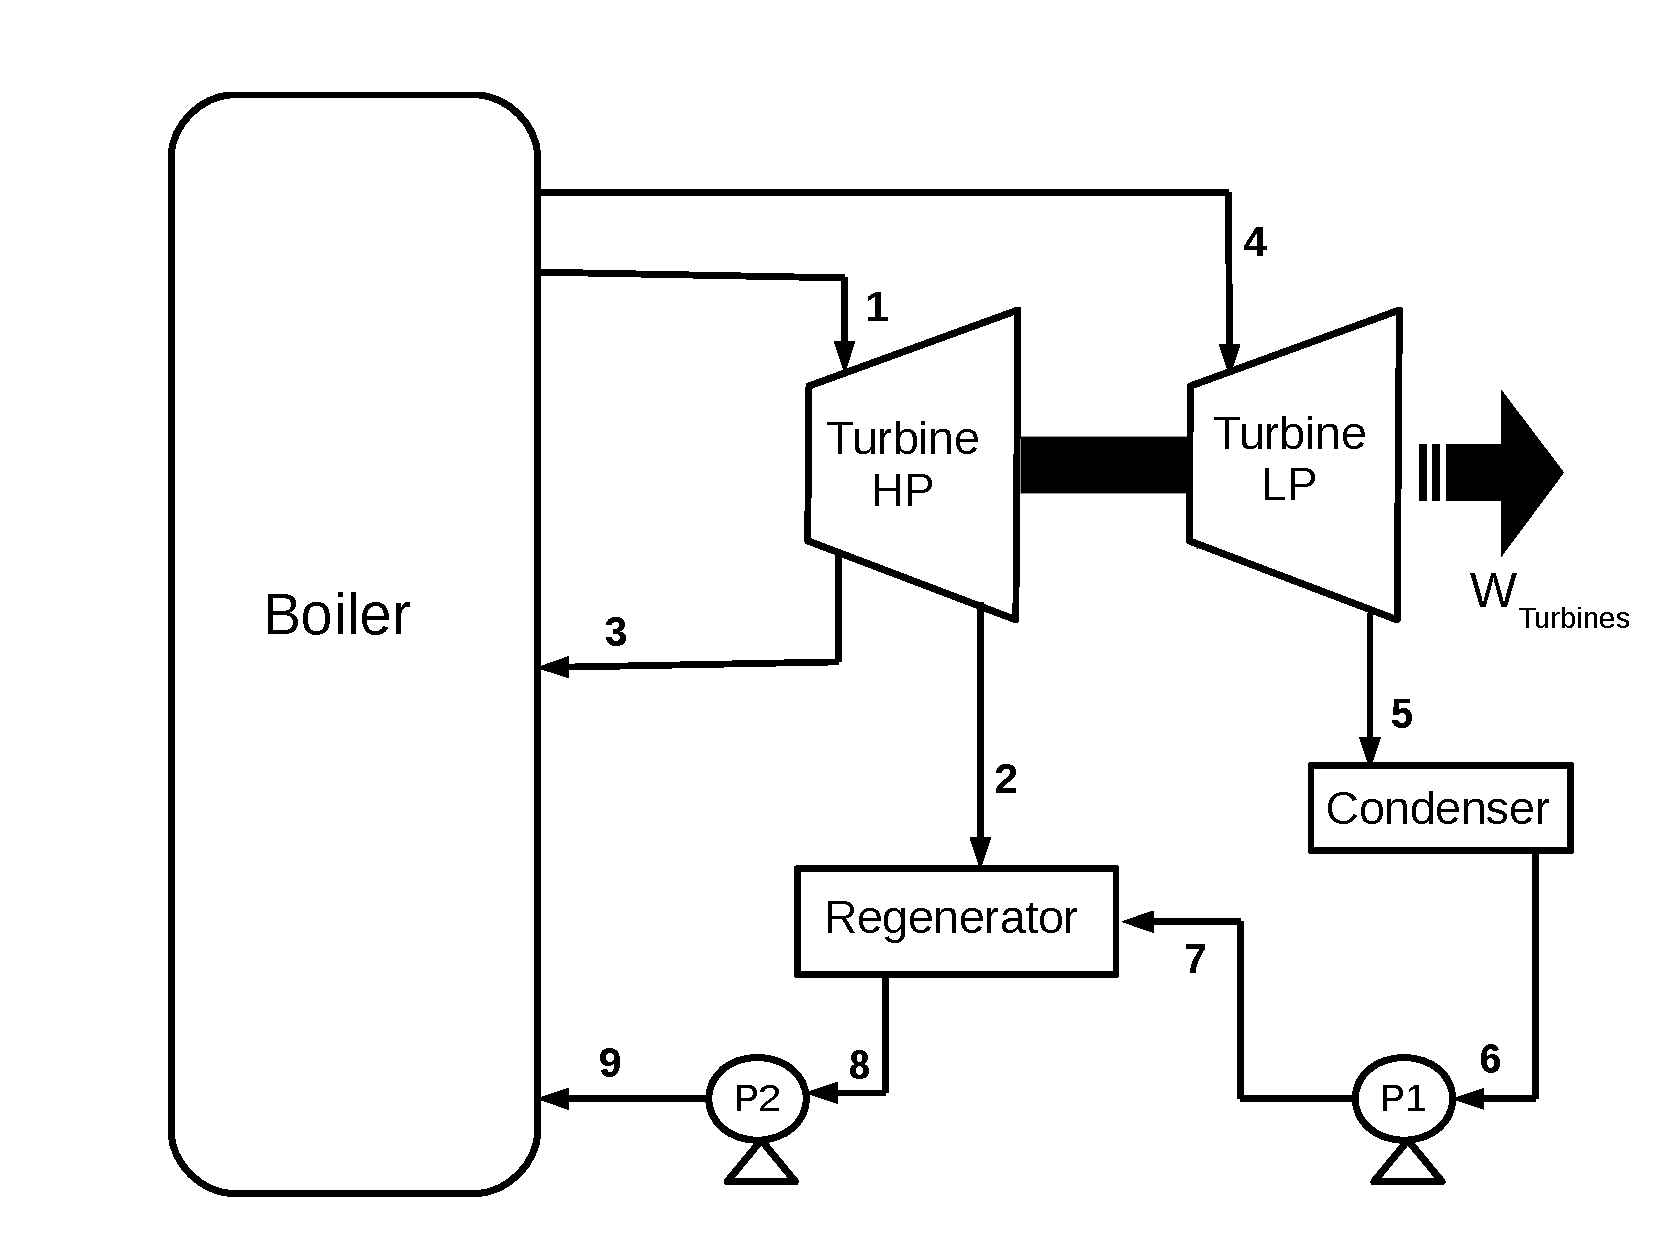
\includegraphics[width=8.cm,clip]{./Pics/Exam_Reheat_Regenerative_Rankine_Cycle}
\caption{ Reheat and regenerative Rankine cycle with 2 turbines.}
\label{exam_mod02_rankinecycle}
\end{center}
\end{figure}

\begin{table}[!h]
\caption{Thermodynamic table of the reheat and regenerative Rankine cycle.}% (Question 1).}
\begin{center}
\begin{tabular} {||c | c c c c c c || }
\hline\hline
{\bf Stage} & {\bf P}    & {\bf T}        & {\bf State}    & {\bf H}             & {\bf S}                  & {\bf Steam}\\
            & {\bf (bar)}& {\bf ($^{o}$C)} &               & {\bf (kJ.kg$^{-1}$)} & {\bf (kJ.(kg.K)$^{-1}$)}  & {\bf Quality}\\
\hline\hline
 {\bf 1 }   & 120        & 565            &   {\bf (a)}    & {\bf (b)}           & {\bf (c)}                & --          \\
 {\bf 2 }   & 3          &  --            &   wet vapour   & {\bf (d)}           &   --                     & {\bf (e)}   \\
 {\bf 3 }   & 3          & 250            &   --           & --                  & --                       & --           \\
 {\bf 4 }   & 3          & 475            &   --           & --                  & --                       & --            \\
 {\bf 5 }   & 0.06       & --             &   wet vapour   & {\bf (f)}           & --                       & {\bf (g)}     \\
 {\bf 6 }   & --         & --             &   sat.liquid   & {\bf (h)}           & --                       & -- \\
 {\bf 7 }   & 3          & --             &   --           & {\bf (i)}           & --                       & --     \\
 {\bf 8 }   & 3          & --             &   --           & --                  & --                       & --           \\
 {\bf 9 }   & 120        & --             &   --           & {\bf (j)}           &  --                      & -- \\
\hline\hline
\end{tabular}
\end{center}
\label{exam1_table1}
\end{table}


\begin{enumerate}[(a)]
\item In Table \ref{exam1_table1}, determine {\it (a)-(j)}. ~\marks{10}%{\bf [10 Marks]}
%
\solution{In order to fill the Table we need to calculate the thermodynamic properties for each stage of the cycle:
\begin{description}
%%%
\item [Stage 1:] The fluid leaving the boiler towards the first turbine is at 120 bar and 565$^{o}$C. This is well above the saturation temperature $\left(T_{\text{sat}}=324.60^{\text{o}}\text{C}\right)$ and we can thus confirm that the fluid is superheated steam~\solmarks{1/10}. At such pressure, the superheated steam tables (SHST) results in (through linear interpolation):\\
 $H_{1}=3518.77\frc{kJ}{kg}$~\solmarks{1/10} and\\
 $S_{1}=6.6983\frc{kJ}{kg.K}$~\solmarks{1/10}.

%%%
\item [Stage 2:] Isentropic expansion in {\it HP Turbine} at $P_{2}=3\;\text{bar} \Leftrightarrow \;\; S_{2}=S_{1}=6.6983\frc{kJ}{kg.K}$. The fluid is at wet vapour state. The quality of the steam is~\solmarks{1/10}
\begin{displaymath}
x_{2}=\frc{S_{2}-S_{f}}{S_{g}-S_{f}}=\frc{6.6983-1.6716}{6.9909-1.6716}=0.9450
\end{displaymath}
Now calculating the enthalpy,~\solmarks{1/10}
\begin{displaymath}
x_{2}=\frc{H_{2}-H_{f}}{H_{g}-H_{f}}=0.9450 \Leftrightarrow H_{2}=2605.72\frc{kJ}{kg}
\end{displaymath}

%%%
\item [Stage 3:] The fluid at $P_{3}=P_{2}=3.0\;\text{bar}$ and $T_{3}=250^{\text{o}}C \left(>> T_{\text{sat}}=133.5^{\text{o}}C\right)$ is superheated steam with $H_{3}=2967.6\frc{kJ}{kg}$ and $S_{3}=7.517\frc{kJ}{kg.K}$.

%%%
\item [Stage 4:] The steam leaves the boiler towards the LP turbine at $P_{4}=P_{3}=3.0\;\text{bar}$ and $T_{4}=475^{\text{o}}C$ (also as superheated steam) with (via linear interpolation) $H_{4}=3433.33\frc{kJ}{kg}$ and $S_{4}=8.252\frc{kJ}{kg}$.

%%%
\item [Stage 5:] Isentropic expansion with $P_{5}=0.060\;\text{bar}$ $\left(\text{with }S_{5}=S_{4}\right)$. The quality of the steam is~\solmarks{1/10}
\begin{displaymath}
x_{5}=\frc{S_{5}-S_{f}}{S_{g}-S_{f}}=\frc{8.252-0.521}{8.330-0.521}=0.99 
\end{displaymath}
and the enthalpy,~\solmarks{1/10}
\begin{displaymath}
x_{5}=0.99=\frc{H_{5}-H_{f}}{H_{g}-H_{f}}=\frc{H_{5}-151.5}{2567.4-151.5}\Leftrightarrow H_{5}=2543.24\frc{kJ}{kg} 
\end{displaymath}

%%%
\item [Stage 6:] The fluid leaves the condenser at $P_{6}=P_{5}=0.06\;\text{bar}$ is saturated liquid with $H_{6}$=$H_{f}\left(0.06\;\text{bar}\right)=151.5\frc{kJ}{kg}$~\solmarks{1/10}

%%%
\item [Stage 7:] Saturated and incompressible liquid leaving the pump towards the regenerator at $P_{7}=P_{2}=3.0\;\text{bar}$,~\solmarks{1/10}
\begin{eqnarray}
H_{7}&\approx& H_{6} + V_{6}\left(P_{7}-P_{6}\right) \nonumber \\
                     &\approx& 151.5 \frc{kJ}{kg} + 0.001006 \frc{m^{3}}{kg}\left(3-0.06\right)\text{bar} \times \frc{10^{5} \frc{N}{m^{2}}}{1\text{ bar}} \times \frc{1\text{ J}}{1\text{ N.m}} \times \frc{10^{-3}\text{ kJ}}{1\text{ J}} \nonumber \\
%kg/\left(m.s^{2}\right)}{1\text{ bar }} \times \frc{10^{-3} \frc{kJ}{kg}}{m^{2}/s^{2}}\times \frc{1}{0.61} \nonumber \\
     &\approx& 151.795\;\frc{kJ}{kg} \nonumber
\end{eqnarray}

%%%
\item [Stage 8:] Saturated liquid water leaving the regenerator at $P_{8}=3.0\;\text{bar}$ with $H_{8}=H_{f}\left(3.0\;\text{bar}\right)=561.4\frc{kJ}{kg}$ and $V_{8}=0.001068\frc{m^{3}}{kg}$.

%%%
\item[Stage 9:] Saturated and incompressible liquid at $P_{9}=120\;\text{bar}$,~\solmarks{1/10}
\begin{eqnarray}
H_{9}&\approx& H_{8} + V_{8}\left(P_{9}-P_{8}\right) \nonumber \\
                     &\approx& 561.4 \frc{kJ}{kg} + 0.001068 \frc{m^{3}}{kg}\left(120-3\right)\text{bar}  \times \frc{10^{5} \frc{N}{m^{2}}}{1\text{ bar}} \times \frc{1\text{ J}}{1\text{ N.m}} \times \frc{10^{-3}\text{ kJ}}{1\text{ J}} \nonumber \\
%\times \frc{10^{5} kg/\left(m.s^{2}\right)}{1\text{ bar }} \times \frc{10^{-3} \frc{kJ}{kg}}{m^{2}/s^{2}}\times \frc{1}{0.61} \nonumber \\
     &\approx& 573.97\;\frc{kJ}{kg} \nonumber
\end{eqnarray}

\end{description}

Thus the Table becomes:
\begin{center}
\begin{tabular} {||c | c c c c c c || }
\hline\hline
{\bf Stage} & {\bf P}    & {\bf T}        & {\bf State}    & {\bf H}             & {\bf S}                  & {\bf Steam}\\
            & {\bf (bar)}& {\bf ($^{o}$C)} &               & {\bf (kJ.kg$^{-1}$)} & {\bf (kJ.(kg.K)$^{-1}$)}  & {\bf Quality}\\
\hline\hline
 {\bf 1 }   & 120        & 565            &{\bf Superheated vapour}&{\bf 3518.77}&{\bf 6.6983}              & --          \\
 {\bf 2 }   & 3          &  --            &   wet vapour   &{\bf 2605.72}        &   --                     & {\bf 0.9450}   \\
 {\bf 3 }   & 3          & 250            &   --           & --                  & --                       & --           \\
 {\bf 4 }   & 3          & 475            &   --           & --                  & --                       & --            \\
 {\bf 5 }   & 0.06       & --             &   wet vapour   & {\bf 2543.24}       & --                       & {\bf 0.99}     \\
 {\bf 6 }   & --         & --             &   sat.liquid   & {\bf 151.5}         & --                       & -- \\
 {\bf 7 }   & 3          & --             &   --           & {\bf 151.8}         & --                       & --     \\
 {\bf 8 }   & 3          & --             &   --           & --                  & --                       & --           \\
 {\bf 9 }   & 120        & --             &   --           & {\bf 573.97}        &  --                      & -- \\
\hline\hline
\end{tabular}
\end{center}
}

%
\item Calculate the fraction (as $\%$) of steam supplied to the low-pressure (LP) turbine. ~\marks{2}%{\bf [2 Marks]}
%
\solution{Energy balance in the regenerator, assuming total mass of water of $\left(m_{\text{T}}=\right)$ 1 kg, and that a fraction, $\mathcal{F}$, is bled-off from the HP turbine to the regenerator, and the remaining water-steam, $1-\mathcal{F}$ is conducted back to the boiler
\begin{displaymath}
m_{\text{T}}H_{8} = \mathcal{F} H_{2} + \left(1-\mathcal{F}\right)H_{7} \Rightarrow \mathcal{F} = 0.1669 kg
\end{displaymath}
Thus, $m_{2}=\mathcal{F}=0.1669\text{ kg}$ and $m_{3}=m_{4}=m_{5}=m_{6}=m_{7}=\left(1-\mathcal{F}\right)=0.833\text{ kg}$ $\Longrightarrow$ 83.3$\%$ of the steam was supplied to the LP turbine.~\solmarks{2/2}
}
%
\item Determine the heat supplied by the boiler. ~\marks{2}%{\bf [2 Marks]}
%
\solution{The heat supplied by the boiler $\left(Q_{\text{Boiler}}\right)$ can be calculated through the energy balance,~\solmarks{2/2}
\begin{displaymath}
Q_{\text{Boiler}}=\left[m_{\text{T}} H_{1} + \left(1-\mathcal{F}\right)H_{4}\right] - \left[\left(1-\mathcal{F}\right)H_{3}+m_{\text{T}}H_{9}\right] \Rightarrow Q_{\text{Boiler}}=3332.75 \frc{kJ}{kg}
\end{displaymath}
}
%
\item Determine the thermal efficiency of the cycle, ~\marks{6}%{\bf [6 Marks]}
\begin{displaymath}
\eta=\frc{W_{Total}}{Q_{Boiler}} = \frc{\sum W_{\text{Turbines}} - \sum W_{\text{Pumps}}}{Q_{Boiler}}
\end{displaymath} 
%
\solution{Now, in order to calculate the thermal efficiency of the cycle,
\begin{displaymath}
\eta=\frc{W_{Total}}{Q_{Boiler}} = \frc{\sum W_{\text{Turbines}} - \sum W_{\text{Pumps}}}{Q_{\text{Boiler}}}
\end{displaymath} 
We need to calculate the work associated with the turbines and pumps.
\begin{description}
%
\item [HP Turbine:] $W_{\text{T,HP}}=m_{\text{T}}H_{1}-\left[\mathcal{F}H_{2}+\left(1-\mathcal{F}\right)H_{3}\right]=611.86\frc{kJ}{kg}$~\solmarks{1/6}% \textcolor{blue}{(1 Mark)}
%
\item [LP Turbine:] $W_{\text{T,LP}}=\left(1-\mathcal{F}\right)\left(H_{4}-H_{5}\right) = 741.44\frc{kJ}{kg}$~\solmarks{1/6}% \textcolor{blue}{(1 Mark)}
%
\item [Pump 1:] $W_{\text{P,1}}= \left(1-\mathcal{F}\right)\left(H_{7}-H_{6}\right)= 0.246\frc{kJ}{kg}$~\solmarks{1/6}% \textcolor{blue}{(1 Mark)}
%
\item [Pump 2:] $W_{\text{P,2}}= m_{\text{T}} \left(H_{9}-H_{8}\right) = 12.57\frc{kJ}{kg}$\solmarks{1/6}% \textcolor{blue}{(1 Mark)}
%
\end{description}

Thus the thermal efficiency of the cycle is,~\solmarks{2/6}
\begin{displaymath}
\eta = \frc{\sum W_{\text{Turbines}} - \sum W_{\text{Pumps}}}{Q_{\text{Boiler}}} = \frc{1339.76}{3332.27} = 0.4022% \;\;\textcolor{blue}{(2 Marks)} 
\end{displaymath}

}
%
\end{enumerate}

To solve this problem, you should assume that the saturated liquid streams are incompressible, and therefore $dH = VdP$ (where $H$, $V$ and $P$ are enthalpy, volume and pressure, respectively). Quality of the steam is expressed as
\begin{displaymath}
x_{j} = \frc{\Psi_{j}-\Psi_{f}}{\Psi_{g}-\Psi_{f}}\;\;\;\text{with }\Psi=\left\{H,S\right\}
\end{displaymath}


\end{question}


\clearpage


%%%
%%% Question 2
%%%
\begin{question}
Refrigerant R-134a is used in a geothermal heat pump system (Fig. \ref{Exam01_Prob4}) to a storage in an industrial facility at 40$^{\text{o}}$C. The heat pump uses underground water from a well to produce a heating capacity of 6 tons. Determine:
\begin{figure}[!h]
\begin{center}
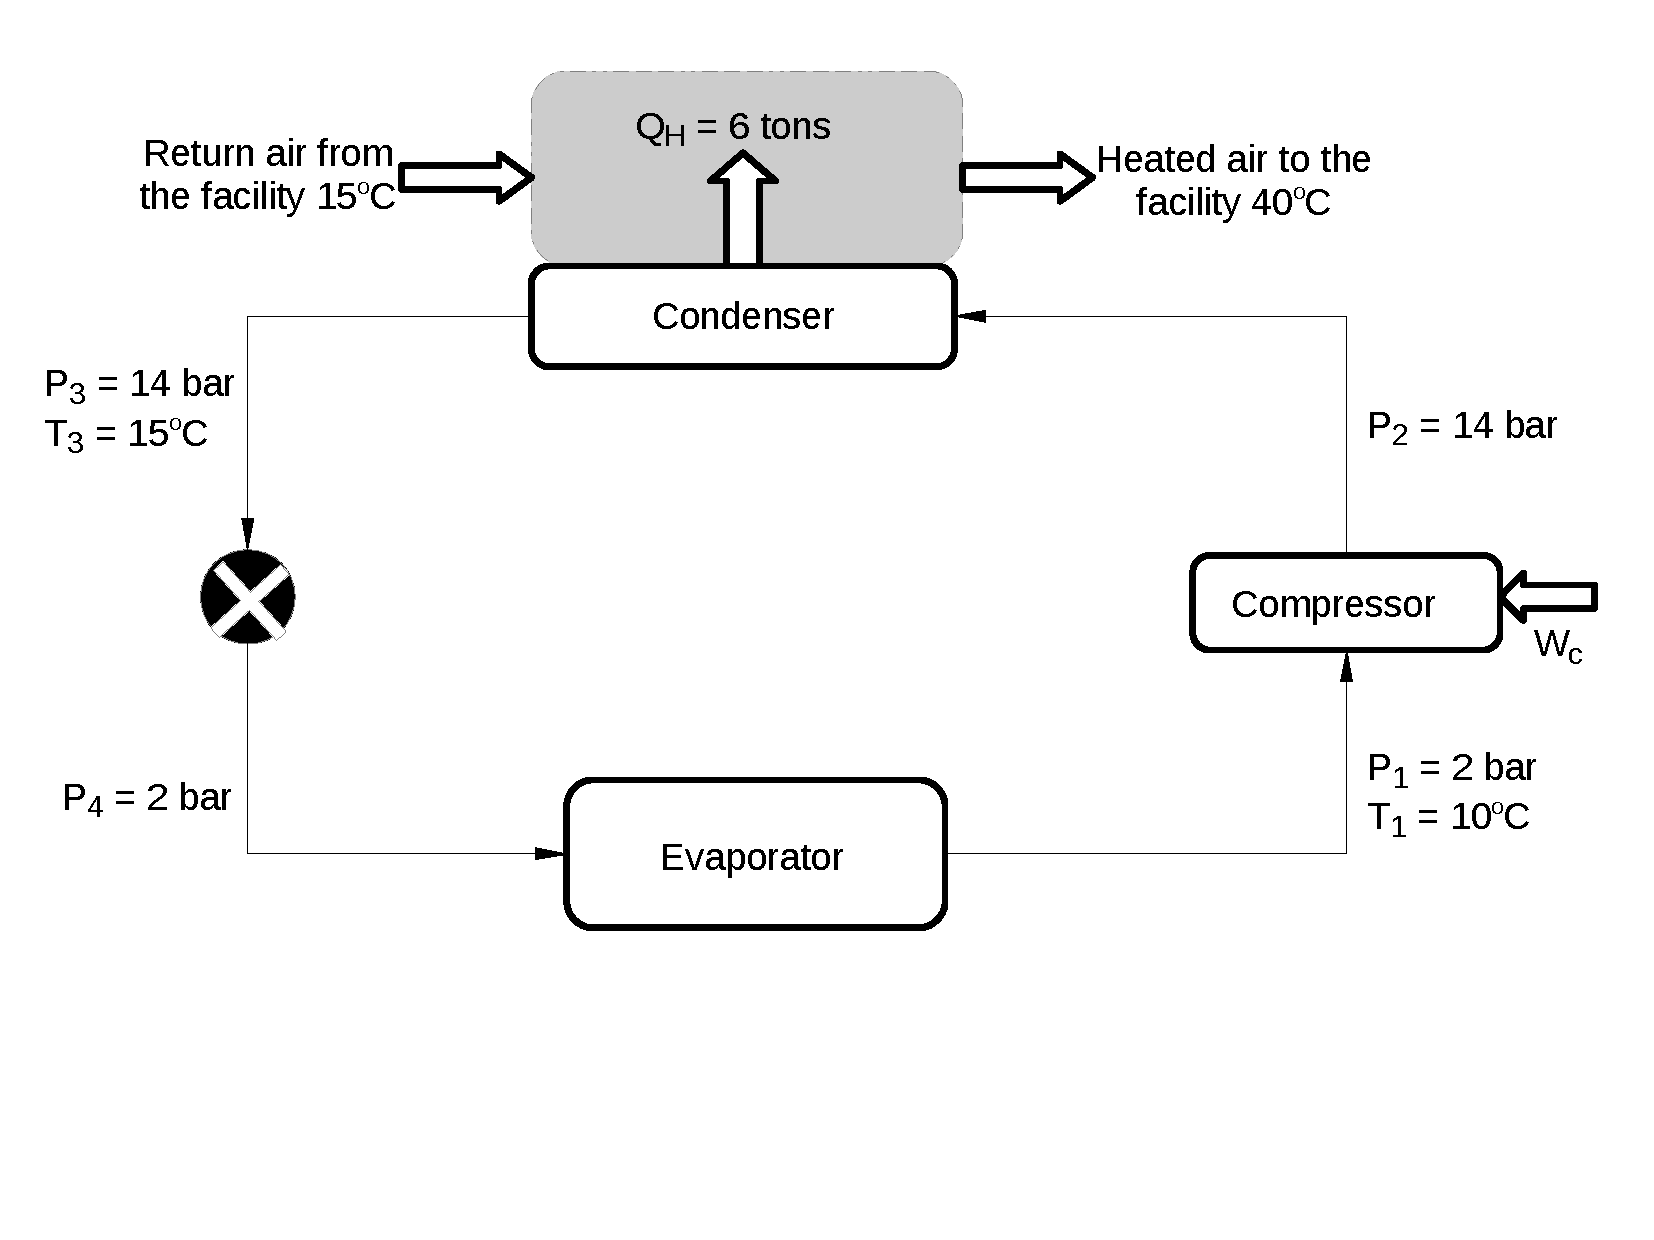
\includegraphics[width=12.0cm,height=9.0cm]{./Pics/Overview_Refrig42}
\end{center}
\vspace{-2.8cm}
\caption{Heat pump cycle.}\label{Exam01_Prob4}
\end{figure}
\begin{enumerate}
 \item Enthalpies and Entropies: H$_{i}$, S$_{i}$ with $i=\left\{1,2,3,4\right\}$;~\marks{8}% {\bf[8 Marks]}
%%
\solution{Calculating all enthalpies and entropies of the cycle:
\begin{description}
%%%
\item [Stage 1:] The refrigerant fluid leaves the evaporator at $P_{1}= 2\;\text{bar}$ and $T_{1}=10^{\text{o}}C >> T_{\text{sat}}=-10.09^{\text{o}}C$, thus the fluid is at {\it superheated vapour} state and with $H_{1}=258.89\frc{kJ}{kg}$ and $S_{1}=0.9898\frc{kJ}{kg.K}$~\solmarks{2/8}.

%%%
\item [Stage 2:] Isentropic compression, $S_{2}=S_{1}$, and assuming ideal compressor at $P_{2}=14\;\text{bar}$. Via linear interpolation, $H_{2}=303.66\frc{kJ}{kg}$~\solmarks{2/8} and $T_{2}=77.08^{\text{o}}C$.

%%%
\item [Stage 3:] The fluid leaves the condenser at $P_{3}=14\;\text{bar}$ and $T_{3}=15^{\text{o}}C\left( << T_{\text{sat}}=52.4^{\text{o}}C\right)$ is a {\it sub-cooled liquid} with $H_{3}=125.26\frc{kJ}{kg}$ and $S_{3}=0.4453\frc{kJ}{kg.K}$~\solmarks{2/8}.

%%%
\item [Stage 4:] Isenthalpic process, $H_{4}=H_{3}$~\solmarks{2/8}, at $P_{4}=2\;\text{bar}$. Calculating the quality of the vapour,
\begin{displaymath}
x_{4}=\frc{H_{4}-H_{f}}{H_{g}-H_{f}}=\frc{125.26-36.84}{241.30-36.84}=0.4325
\end{displaymath}
and the entropy,
\begin{displaymath}
x_{4}=\frc{S_{4}-S_{f}}{S_{g}-S_{f}}=\frc{S_{4}-0.1481}{0.9253-0.1481} \Rightarrow S_{4}=0.4842\frc{kJ}{kg.K}
\end{displaymath}
%%%
\end{description}
}
%
 \item Volumetric flow rate of heated air to the room $\left(m^{3}/s\right)$;~\marks{3}% {\bf[3 Marks]}
%
\solution{In order to calculate the volumetric flow rate of heated air, we first need to determine the mass flow rate,~\solmarks{1/3}
\begin{eqnarray}
&&Q_{H} = \dot{m}_{\text{air}}\left(H_{\text{out}}^{\text{air}}-H_{\text{in}}^{\text{air}}\right) = \dot{m}_{\text{air}}C_{p}^{\text{air}}\left(T_{\text{out}}^{\text{air}}-T_{\text{in}}^{\text{air}}\right) \nonumber \\
&&6\;\text{ton} \times \frc{210\frc{kJ}{\text{min}}}{1\;\text{ton}}\times\frc{1\text{ min }}{60s}=\dot{m}_{\text{air}}\times 1.004\frc{kJ}{kg.K}\left(40-15\right)^{\text{o}}C\nonumber \\
&&\dot{m}_{\text{air}} =0.8367 \frc{kg}{s} \nonumber 
\end{eqnarray}

Now for the volumetric flow rate $\left(\text{with }T=40^{\text{o}}C\right.$ and $\left.P=1.01325\text{ bar}\right)$~\solmarks{2/3}
\begin{eqnarray}
\dot{V}_{\text{air}}^{\text{out}}&=&\dot{m}_{\text{air}}V_{\text{air}}^{\text{out}}=\dot{m}_{\text{air}}\frc{RT_{\text{air}}^{\text{out}}}{P_{\text{air}}} \nonumber \\
                             &=&0.8367\frc{\text{kg}}{s} \times 287 \frc{\text{J}}{\text{kg.K}} \times \frc{\left(40 + 273.15\right)\text{ K}}{1.0125\text{ bar}} \times \frc{1\text{ N.m}}{1\text{ J}} \times \frc{1\text{ bar}}{10^{5}\text{ N/m}^{2}} \nonumber \\ 
                             &=& 0.7426 \frc{m^{3}}{s} \nonumber 
\end{eqnarray}
}
%
 \item Mass flow rate of the R-134a refrigerant fluid;~\marks{3}% {\bf[3 Marks]}
%
\solution{The mass flow rate of the refrigerant fluid R-134a can be calculated as,~\solmarks{3/3}
\begin{displaymath}
Q_{H}=\dot{m}_{R}\left(H_{2}-H_{3}\right)\Rightarrow \dot{m}_{R}=0.1177\frc{kg}{s}
\end{displaymath}
}
%
 \item Compressor power $\left(W_{C}\right)$ in kW;~\marks{3}% {\bf[3 Marks]}
%
\solution{~\solmarks{3/3}
\begin{displaymath}
W_{C}=\dot{m}_{R}\left(H_{2}-H_{1}\right)\Rightarrow W_{C}=5.27\;kW
\end{displaymath}
}
%
 \item Coefficient of performance $\left(\text{COP}=\frc{Q_{H}}{W_{C}}\right)$;~\marks{3}% {\bf[3 Marks]}
%
\solution{~\solmarks{3/3}
\begin{displaymath}
\text{COP} = \frc{Q_{H}}{W_{C}}=3.98
\end{displaymath}
}
%
\end{enumerate}
Given the heat capacity, $C_{p}^{\text{air}}=1.004\;kJ.\left(kg.K\right)^{-1}$, and molecular weight, $MW^{\text{air}}=28.97\;kg.kgmol^{-1}$ of air. Assume that air behaves as an ideal gas. Quality of the vapour is expressed as
\begin{displaymath}
x_{j} = \frc{\Psi_{j}-\Psi_{f}}{\Psi_{g}-\Psi_{f}}\;\;\;\text{with }\Psi=\left\{H,S\right\}
\end{displaymath}


\end{question}

\clearpage

%%%%%%%%%%%%%%%%%%%%%%%%%%
%%%% Question 01       %%%
%%%%%%%%%%%%%%%%%%%%%%%%%%
%\begin{question}
%\begin{enumerate}[(a)]
%%%%%%%%%%%%%%%%%%%%%%%%%%%
%\item ~\marks{3}
%\solution{
%}
%
%%%%%%%%%%%%%%%%%%%%%%%%%%%
%\item ~\marks{3}
%\solution{
%}
%\end{enumerate}
%\end{question}
%
%\clearpage
%
%%%%%%%%%%%%%%%%%%%%%%%%%%
%%%% Question 02       %%%
%%%%%%%%%%%%%%%%%%%%%%%%%%
%\begin{question} 
%\begin{enumerate}[(a)]
%%%%%%%%%%%%%%%%%%%%%%%%%%%
%\item ~\marks{3}
%\solution{
%}
%
%%%%%%%%%%%%%%%%%%%%%%%%%%%
%\item ~\marks{3}
%\solution{
%}
%\end{enumerate}
%\end{question}
%\clearpage

%%%%%%%%%%%%%%%%%%%%%%%%%
%%% Question 03       %%%
%%%%%%%%%%%%%%%%%%%%%%%%%
\begin{question} 

A steady flow energy device formed of a turbine with one inlet (labelled 1), and two outlets (labelled 2 and 3), does work on an ideal gas at a rate of $120$\,kW. The specific gas constant $R=287$\,J\,kg$^{-1}$\,K$^{-1}$ and the specific heat capacity at constant pressure $c_p=1003$\,J\,kg$^{-1}$\,K$^{-1}$, while the known conditions at the inlet and each outlet are given in table~\ref{tab:multiInletOutlet}.

%%%%%%%%%%%%%%%%%%%%%%%%%%%%%%%%%%
\begin{table}[!h]
\caption{Inlet and outlet conditions for the steady flow device}
\label{tab:multiInletOutlet}
\begin{center}
\begin{tabular}{| c || c | c | c | c | c |} \hline
Inlet/Outlet & Area       & Volume flux          & Temperature    & Pressure & Height  \\
             & $A$ (m$^2$) & $q$ (m$^3$\,s$^{-1}$) & $T$ ($^\circ$C) & $p$ (Pa)  & $z$ (m)  \\ \hline
$1$          & $0.1$      & $2.0$                & $20$           & $p_{1}$     & $0.0$   \\
$2$          & $0.1$      & $1.0$                & $50$           & $200000$ & $10.0$ \\
$3$          & $0.05$     & $1.0$                & $90$           & $100000$ & $4.0$  \\
\hline
\end{tabular}
\end{center}
\end{table}

\begin{enumerate}[(a)]
%%%%%%%%%%%%%%%%%%%%%%%%%%
\item The steady flow energy equation for a steady flow device with one inlet and one outlet is
\begin{align*}
 \frac{\dot{Q} - \dot{W}_s}{\dot{m}} = \left(c_p T_\text{outlet} + \frac{u_\text{outlet}^2}{2} + g z_\text{outlet}\right) - \left(c_p T_\text{inlet} + \frac{u_\text{inlet}^2}{2} + g z_\text{inlet}\right),
\end{align*}
where $u$ is the gas velocity, $\dot{Q}$ is the rate of heat addition and $\dot{W}_s$ is the rate at which shaft work is done on the gas. Explain how this equation should be changed to model the device described above.~\marks{4}
\solution{The mass flux entering the device $\dot{m}_1$ is now divided between two outlets. Therefore the modified mass conservation equation would be
\begin{align*}
 \dot{m}_1 = \dot{m}_2 + \dot{m}_3.
\end{align*}~\solmarks{1/4}

With two outlets, the flux of energy must also be split between the two outlets, which gives
\begin{align*}
 \dot{Q} - \dot{W}_s = \dot{m}_2 \left(c_p T_2 + \frac{u_2^2}{2} + g z_2\right) + \dot{m}_3 \left(c_p T_3 + \frac{u_3^2}{2} + g z_3\right) - \dot{m}_1 \left(c_p T_1 + \frac{u_1^2}{2} + g z_1\right).
\end{align*}~\solmarks{3/4}
}

%%%%%%%%%%%%%%%%%%%%%%%%%%
\item Calculate the gas velocity at the inlet and each outlet;~\marks{3}
\solution{The gas velocities are given by
\begin{align*}
 u_1 =& \frac{q_1}{A_1} = \frac{2.0\,\mbox{m}^3\,\mbox{s}^{-1}}{0.1\,\mbox{m}^2} = 20\,\mbox{m\,s}^{-1}, \\
 u_2 =& \frac{q_2}{A_2} = \frac{1.0\,\mbox{m}^3\,\mbox{s}^{-1}}{0.1\,\mbox{m}^2} = 10\,\mbox{m\,s}^{-1}, \\
 u_3 =& \frac{q_3}{A_3} = \frac{1.0\,\mbox{m}^3\,\mbox{s}^{-1}}{0.05\,\mbox{m}^2} = 20\,\mbox{m\,s}^{-1}.
\end{align*}~\solmarks{3/3}
}

%%%%%%%%%%%%%%%%%%%%%%%%%%
\item Determine the pressure at the inlet $\left(p_{1}\right)$;~\marks{5}
\solution{
The densities at the outlets can be obtained via the ideal gas equation
\begin{align*}
 \rho_2 =& \frac{p_2}{R T_2} = \frac{200000 \,\mbox{Pa}}{287\,\mbox{J\,kg}^{-1}\,\mbox{K}^{-1}\left(50+273.15\right)\,\mbox{K}} = 2.1564726\,\mbox{kg\,m}^{-3}, \\
 \rho_3 =& \frac{p_3}{R T_3} = \frac{100000 \,\mbox{Pa}}{287\,\mbox{J\,kg}^{-1}\,\mbox{K}^{-1} \left(90+273.15\right)\,\mbox{K}} = 0.9594714\,\mbox{kg\,m}^{-3}.
\end{align*}~\solmarks{2/5}
 
Mass conservation gives $\dot{m}_1 = \dot{m}_2 + \dot{m}_3$ where the mass flux $\dot{m} = \rho q$. Therefore
\begin{align*}
 \rho_1 = \frac{\rho_2 q_2 + \rho_3 q_3}{q_1} =& \frac{\left(2.1564726\,\mbox{kg\,m}^{-3} \times 1\,\mbox{m}^3\,\mbox{s}^{-1}\right) + \left(0.9594714\,\mbox{kg\,m}^{-3} \times 1\,\mbox{m}^3\,\mbox{s}^{-1}\right)}{2\,\mbox{m}^3\,\mbox{s}^{-1}} \nonumber \\
 =& 1.557972\,\mbox{kg\,m}^{-3}
\end{align*}~\solmarks{2/5}

The pressure at the inlet is now
\begin{align*}
 p_1 = \rho_1 R T_1 = 1.557972\,\mbox{kg\,m}^{-3} \times 287\,\mbox{J\,kg}^{-1}\,\mbox{K}^{-1} \times \left(20 + 273.15\right)\,\mbox{K} = 131078.49\,\mbox{Pa}. 
\end{align*}~\solmarks{1/5}
}

%%%%%%%%%%%%%%%%%%%%%%%%%%
\item What is the relative percentage error if the gravitational potential energy terms are neglected when calculating the rate of heat transfer $\dot{Q}$?~\marks{8}
\solution{
The mass fluxes at each inlet and exit are
\begin{align*}
 \dot{m}_1 =& \rho_1 q_1 = 1.557972\,\mbox{kg\,m}^{-3} \times 2\,\mbox{kg/s} = 3.1159440\,\mbox{kg/s}, \\
 \dot{m}_2 =& \rho_2 q_2 = 2.1564726\,\mbox{kg\,m}^{-3} \times 1\,\mbox{kg/s} = 2.1564726\,\mbox{kg/s}, \\
 \dot{m}_3 =& \rho_3 q_3 = 0.9594714\,\mbox{kg\,m}^{-3} \times 1\,\mbox{kg/s} = 0.9594714\,\mbox{kg/s}.
\end{align*} \solmarks{1/8}

The energy fluxes without gravitational potential energy are
\begin{align*}
 c_p T_1 + \frac{u_1^2}{2} =& 294229.45\,\mbox{m}^2/\mbox{s}^2, \\
 c_p T_2 + \frac{u_2^2}{2} =& 324169.45\,\mbox{m}^2/\mbox{s}^2, \\
 c_p T_3 + \frac{u_3^2}{2} =& 364439.45\,\mbox{m}^2/\mbox{s}^2. 
\end{align*} \solmarks{1/8}

The energy fluxes with gravitational potential energy are
\begin{align*}
 c_p T_1 + \frac{u_1^2}{2} + g z_1 =& 294229.45\,\mbox{m}^2/\mbox{s}^2, \\
 c_p T_2 + \frac{u_2^2}{2} + g z_2 =& 324267.55\,\mbox{m}^2/\mbox{s}^2, \\
 c_p T_3 + \frac{u_3^2}{2} + g z_3 =& 364478.69\,\mbox{m}^2/\mbox{s}^2.
\end{align*} \solmarks{1/8}

The rate of heat addition without gravitational potential energy is
\begin{align*}
 \dot{Q}_\text{with} =& \dot{W}_s + \dot{m}_2 \left(c_p T_2 + \frac{u_2^2}{2}\right) + \dot{m}_3 \left(c_p T_3 + \frac{u_3^2}{2}\right) - \dot{m}_1 \left(c_p T_1 + \frac{u_1^2}{2}\right) \\
 =& -120000 + 699062.53 + 349669.25 - 916802.49\\
 =& 11929.28\,\mbox{W}.
\end{align*}
Note turbine does work on gas so $\dot{W}_s$ is negative. \solmarks{2/8}

The rate of heat addition with gravitational potential energy is
\begin{align*}
 \dot{Q}_\text{without} =& \dot{W}_s + \dot{m}_2 \left(c_p T_2 + \frac{u_2^2}{2} + g z_2\right) + \dot{m}_3 \left(c_p T_3 + \frac{u_3^2}{2} + g z_3\right) - \dot{m}_1 \left(c_p T_1 + \frac{u_1^2}{2} + g z_1\right) \\
 =& -120000 + 699274.08 + 349706.9 - 916802.49\\
 =& 12178.48 \,\mbox{W}.
\end{align*} 
Note turbine does work on gas so $\dot{W}_s$ is negative. \solmarks{2/8}

The relative percentage difference between the rate of heat addition with and without the gravitational potential energy terms is
\begin{align*}
 100\% \abs{\frac{\dot{Q}_\text{with} - \dot{Q}_\text{without}}{\dot{Q}_\text{with}}} =& 100\% \abs{\frac{12178.48 - 11929.28}{12178.48}} = 2.0462\%. 
\end{align*} \solmarks{1/8}
}
\end{enumerate}
\end{question}

\clearpage


%%%%%%%%%%%%%%%%%%%%%%%%%
%%% Question 04       %%%
%%%%%%%%%%%%%%%%%%%%%%%%%
\begin{question} 

\begin{enumerate}[(a)]
\item Gas flows along a pipe of slowly varying cross section in the direction of increasing $x$. By considering the rate of change of the mass of gas within a small section of pipe and the gas mass fluxes into and out of this section of pipe, show that
\begin{align*}
 \fracp{}{t}\left(\rho A\right) + \fracp{}{x}\left(\rho u A\right) = 0.
\end{align*}
Here the gas velocity $u$, density $\rho$ and pipe cross section $A$ are all functions of $x$ and time $t$. \marks{5} \\
\solution{The total mass contained in a section of pipe of length $\Delta x$ is $\rho A \Delta x$.  \solmarks{1/5}

The rate of change of mass in this section of pipe equals the mass flux entering the pipe $\rho u A$ minus the mass flux leaving the other end of the pipe section
\begin{align*}
 \rho u A + \Delta x \fracp{}{x}\left(\rho u A\right).
\end{align*}
[Obtained via a linearized Taylor expansion.] \solmarks{2/5}

Hence mass conservation implies
\begin{align*}
 \fracp{}{t}\left(\rho A\right) = \rho u A - \rho u A - \Delta x \fracp{}{x}\left(\rho u A\right).
\end{align*}
and hence dividing by $\Delta x$ and rearranging gives the result. \solmarks{2/5}
}

%%%%%%%%%%%%%%%%%%%%%%%%%%
\item Explain what is meant by a steady flow and show that for steady flow in a pipe of uniform cross section
\begin{align*}
 \frac{1}{\rho} \fracd{\rho}{x} + \frac{1}{u} \fracd{u}{x} = 0.
\end{align*}
~\marks{4}
\solution{The flow is steady if the density, velocity and cross section depend only on $x$ and not time $t$. In this case the result from (a) gives
\begin{align*}
 \fracd{}{x}\left(\rho u A\right) = 0.
\end{align*}~\solmarks{2/4}

If the pipe has uniform cross section, then $A$ is constant. Therefore via the chain rule
\begin{align*}
 \rho \fracd{u}{x} + u \fracd{\rho}{x} = 0.
\end{align*}
Finally dividing by $\rho u$ gives the required result.\solmarks{2/4}
}

%%%%%%%%%%%%%%%%%%%%%%%%%%
\item For steady compressible flow in a uniform pipe, using the conservation of energy and the laws of thermodynamics; changes in the entropy $s$, is related to changes in the pressure pressure $p$, density $\rho$ and velocity $u$, through
\begin{align*}
  T \,\d{s} + \frac{\d{p}}{\rho} + u \, \d{u} = 0.
\end{align*}
Hence show that the change in pressure and the change in entropy as fluid flows are related through
\begin{align*}
 \left(1 - \frac{u^2}{c^2}\right) \fracd{p}{x} = -\rho T \left(1 + \frac{u^2 \beta}{c_p}\right) \fracd{s}{x}.
\end{align*}

In the derivation of this result, you may additionally assume that a change in gas density
\begin{align*}
 \d{\rho} = \frac{\d{p}}{c^2} - \frac{\rho \beta T}{c_p} \d{s},
\end{align*}
where $c$ is the speed of sound, $\beta$ is the thermal expansion coefficient and $c_p$ is the specific heat capacity as constant pressure. \marks{8}
\solution{
Variations over $x$ imply
\begin{align*}
 T \fracd{s}{x} + \frac{1}{\rho} \fracd{p}{x} + u \fracd{u}{x} = 0, \quad \mbox{and} \quad \fracd{\rho}{x} = \frac{1}{c^2} \fracd{p}{x} - \frac{\rho \beta T}{c_p} \fracd{s}{x}.
\end{align*}
Using the second equation, we eliminate the $\fracd{\rho}{x}$ from the mass conservation equation to give
\begin{align*}
 \rho \fracd{u}{x} + \frac{u}{c^2} \fracd{p}{x} - \frac{u \rho \beta T}{c_p} \fracd{s}{x} = 0.
\end{align*}~\solmarks{2/8}

Next we eliminate $\fracd{u}{x}$ to give
\begin{align*}
 \frac{T}{u} \fracd{s}{x} + \frac{1}{\rho u} \fracd{p}{x} = - \fracd{u}{x} = \frac{u}{\rho c^2} \fracd{p}{x} - \frac{u \beta T}{c_p} \fracd{s}{x}.
\end{align*}~\solmarks{2/8}

Collecting all the terms involving $\fracd{p}{x}$ on one side and all the terms involving $\fracd{s}{x}$ on the other side
\begin{align*}
  \frac{1}{\rho u} \fracd{p}{x} - \frac{u}{\rho c^2} \fracd{p}{x} = -\frac{u \beta T}{c_p} \fracd{s}{x} - \frac{T}{u} \fracd{s}{x}.
\end{align*}
\begin{align*}
 \left(\frac{1}{\rho u} - \frac{u}{\rho c^2}\right) \fracd{p}{x} = -T \left(\frac{u \beta}{c_p} + \frac{1}{u}\right) \fracd{s}{x}.
\end{align*}~\solmarks{3/8}

If we multiply by $\rho u$, then
\begin{align*}
 \left(1 - \frac{u^2}{c^2}\right) \fracd{p}{x} = -\rho T \left(1 + \frac{u^2 \beta}{c_p}\right) \fracd{s}{x}.
\end{align*}~\solmarks{1/8}
}

%%%%%%%%%%%%%%%%%%%%%%%%%%
\item Define a Mach number, and (with reference to the result derived in part (c)), explain how the pressure changes as a compressible fluid flows subsonically along a pipe of uniform cross section. \marks{3}
\solution{The Mach number $\Ma$ is the ratio of the actual speed $u$ to the speed of sound $c$, i.e.
\begin{align*}
 \Ma = \frac{u}{c}.
\end{align*} \solmarks{1/3}

For subsonic flow $\Ma < 1$, so the coefficient of $\fracp{p}{x}$ is positive. The density, temperature and velocity are all positive, so the $-\rho T \left(1 + \frac{u^2 \beta}{c_p}\right)$ is negative, while the entropy must increase with flow along the pipe (i.e. $\fracd{s}{x} > 0$). \solmarks{1/3}

Consequently the pressure must fall as fluid flows along the pipe. \solmarks{1/3}
}
\end{enumerate}
\end{question}

\clearpage

%%%%%%%%%%%%%%%%%%%%%%%%%
%%% Question 05       %%%
%%%%%%%%%%%%%%%%%%%%%%%%%
\begin{question} 

\begin{enumerate}[(a)]
%%%%%%%%%%%%%%%%%%%%%%
\item Define the specific humidity $\omega$. Assuming both dry air and water vapour behave like ideal gases with specific gas constants $R_{a}=0.2871$ kJ/(kg.K) and $R_{v}=0.4615$ kJ/(kg.K), respectively, show that
\begin{align*}
\omega = \frac{0.622 p_v}{p-p_v},
\end{align*}
where $p$ is the absolute pressure and $p_{v}$ is the partial pressure of water vapour. \marks{5}
\solution{The specific humidity $\omega$ is the ratio of the mass of water vapour $m_v$ to the mass of dry air $m_a$ in a volume $V$ ~\solmarks{1/5}, i.e.
\begin{align*}
 \omega = \frac{m_v}{m_a}.
\end{align*}~\solmarks{1/5}

In terms of densities
\begin{align*}
 \omega = \frac{\rho_v V}{\rho_a V} = \frac{\rho_v}{\rho_a}.
\end{align*}
Treat both water vapour and dry air as ideal gases, so that
\begin{align*}
 \omega = \frac{p_v}{R_v T}\frac{R_a T}{p_a} = \frac{0.622 p_v}{p_a}.
\end{align*}~\solmarks{2/5}

Finally the partial pressure of water vapour and dry air $p_v + p_a = p$, so
\begin{align*}
 \omega = \frac{0.622 p_v}{p - p_v}.
\end{align*}~\solmarks{1/5}
}

%%%%%%%%%%%%%%%%%%%%%%
\item Define the relative humidity $\varphi$, and hence show that
\begin{align*}
\omega = \frac{0.622 \varphi p_g}{p-\varphi p_g},
\end{align*}
where the saturation pressure of water is denoted $p_g$.~\marks{3}
\solution{The relative humidity $\varphi$ is the ratio of the mass of water vapour $m_v$ to the mass of water vapour at saturation $m_g$, i.e.
\begin{align*}
 \varphi = \frac{m_v}{m_g}.
\end{align*}~\solmarks{1/3}

Again using the ideal gas equation
\begin{align*}
 \varphi = \frac{m_v}{m_g} = \frac{\rho_v V}{\rho_g V} = \frac{p_v}{R_v T}\frac{R_v T}{p_g} = \frac{p_v}{p_g}.
\end{align*}~\solmarks{1/3}

Therefore writing $p_v = \varphi p_g$ in the equation from part (a), gives the required result. \solmarks{1/3}
}


%%%%%%%%%%%%%%%%%%%%%%
\item Air enters an air-conditioning system at 1\,atm, 35$^\circ$C and 60\% relative humidity, at a
rate of 12\,m$^3$/min. Saturated air leaves the air-conditioning system at a temperature of
16$^\circ$C. The moisture in the air that condenses during the process is removed at 16$^\circ$C, while the specific enthalpy of liquid water at 16$^\circ$C is $67.22$\,kJ/kg.

\begin{enumerate}[i)]
\item Determine the rate of moisture removal from the air; \marks{7}
\solution{The inlet and outlet are at $1$\,atm ($=101.325$\,kPa) so we can determine the conditions using the psychrometric chart, which gives
\begin{align*}
 h_1 &= 90\,\mbox{kJ/kg dry air},   &h_2 &= 43\,\mbox{kJ/kg dry air}, \\
 \omega_1 &= 0.022\,\mbox{kg water/kg dry air},   &\omega_2 &= 0.011\,\mbox{kg water/kg dry air}, \\
 V_1 &= 0.905\,\mbox{m}^3\mbox{/ kg dry air}.
\end{align*} \solmarks{3/7}

In the cooling section:
\begin{align*}
\mbox{\textit{Conservation of dry air:}} & & \dot{m}_{a_1} = \dot{m}_{a_2} = \dot{m}_a, \\
\mbox{\textit{Conservation of water vapour:}} & & \dot{m}_{a_1} \omega_1 = \dot{m}_{a_2} \omega_2 + \dot{m}_w, \\
& & ~~ \Rightarrow \dot{m}_w = \dot{m}_a \left(\omega_1 - \omega_2\right).
\end{align*} \solmarks{2/7}

The mass flux of dry air is given by
\begin{align*}
 \dot{m}_a = \frac{\dot{V}_1}{V_1} = \frac{12\,\mbox{m}^3\mbox{/min}}{0.905\,\mbox{m}^3\mbox{/ kg dry air}} = 13.26\,\mbox{kg/min}.
\end{align*} \solmarks{1/7}

Hence the conservation of water vapour gives
\begin{align*}
 \dot{m}_w =& \dot{m}_a \left(\omega_1 - \omega_2\right) \\
 =& 13.26\,\mbox{kg/min} \times \left(0.022 - 0.011\right) \\
 =& 0.15\,\mbox{kg/min}.
\end{align*} \solmarks{1/7}
}

%%%%%%%%%%%%%%%%%%%%
\item Determine the rate of heat removal from the air. \marks{5}
\solution{

In the cooling section:
\begin{align*}
\mbox{\textit{Conservation of energy:}} & & \dot{Q} = \dot{m}_a \left(h_2 - h_1\right) + \dot{m}_w h_w.
\end{align*} \solmarks{1/5}

The heat supplied to the system $\dot{Q}$ is given by the energy conservation equation
\begin{align*}
 \dot{Q} =& \dot{m}_a \left(h_2 - h_1\right) + \dot{m}_w h_w \\
 =& 13.26\,\mbox{kg/min}\left(43 - 90\right)\,\mbox{kJ/kg} + \left(0.15\,\mbox{kg/min} \times 67.22\,\mbox{kJ/kg}\right) \\
 =& -623.204\,\mbox{kJ/min} + 9.804\,\mbox{kJ/min} \\
 =& -613.4\,\mbox{kJ/min}.
\end{align*} \solmarks{3/5}

The rate of heat addition $\dot{Q}$ is negative indicating heat removal from the cooling section. Therefore the rate of heat removal is $613.4$\,kJ/min. \solmarks{1/5}
}

\end{enumerate}

\end{enumerate}
\end{question}

\paperend

%\begin{comment}
\begin{landscape}
%\begin{center}
%\includegraphics[width=1.5\textwidth]{PsychrometricChart}
%\end{center}
{
  \includepdf[pages=-,fitpaper]{./Pics/PsychrometricChart}
  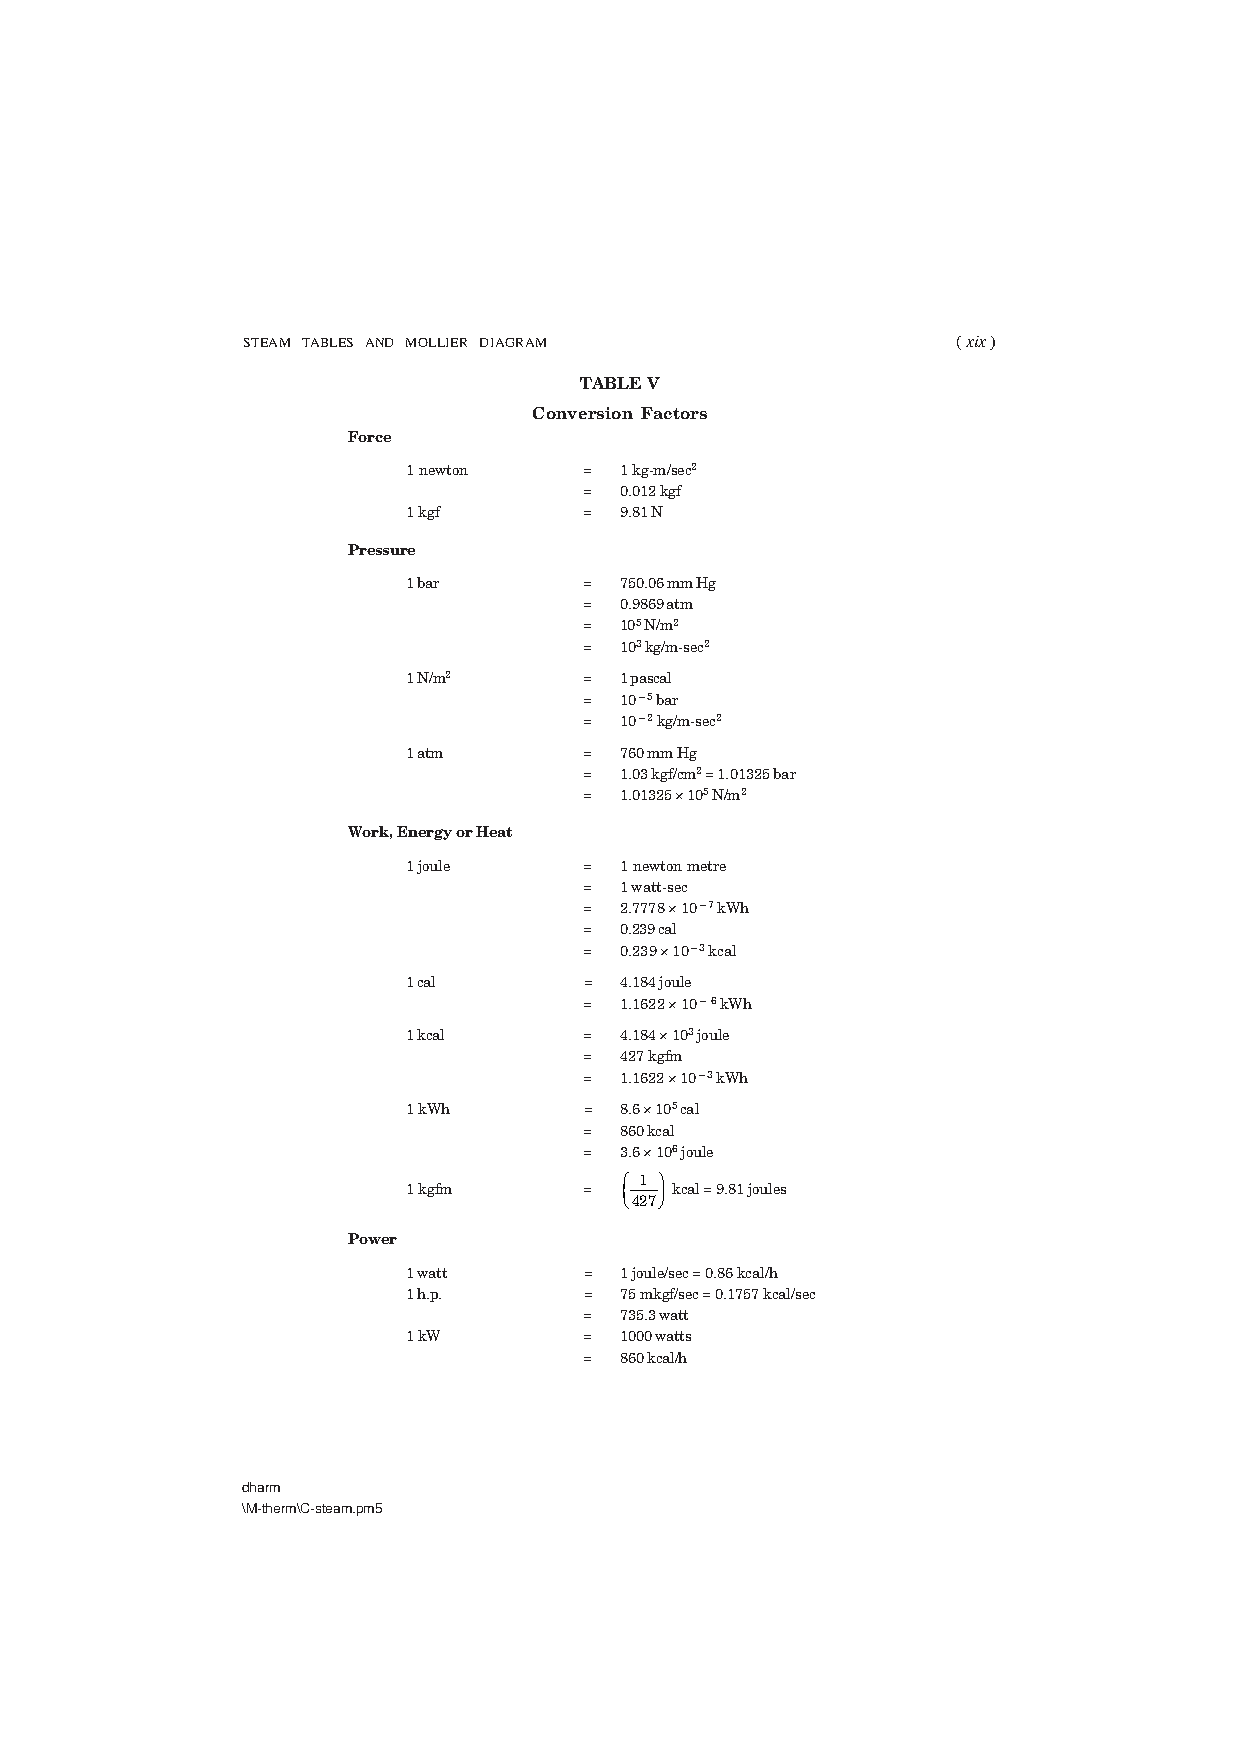
\includepdf[pages=-,fitpaper]{./Pics/UnitsConversion}
  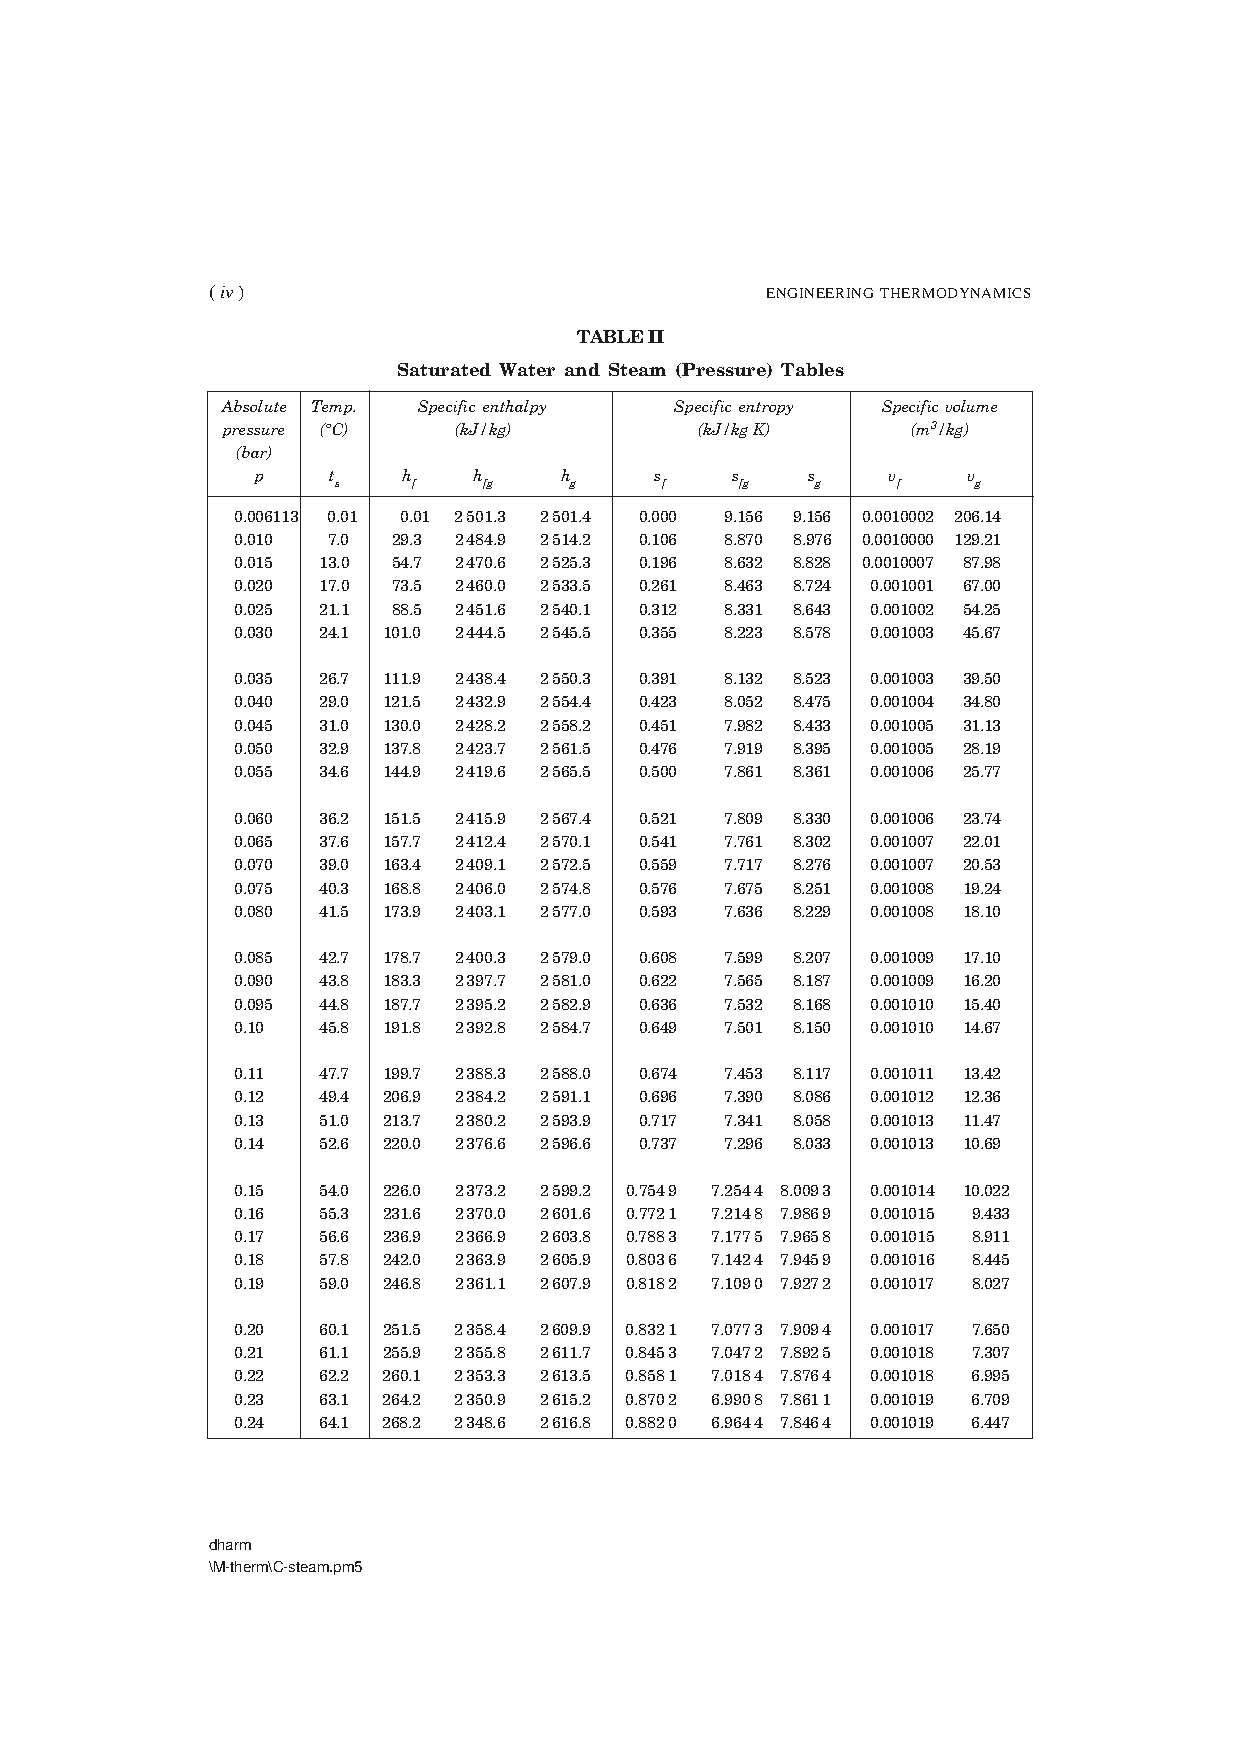
\includepdf[pages=-,fitpaper]{./Pics/SteamTable_2}
  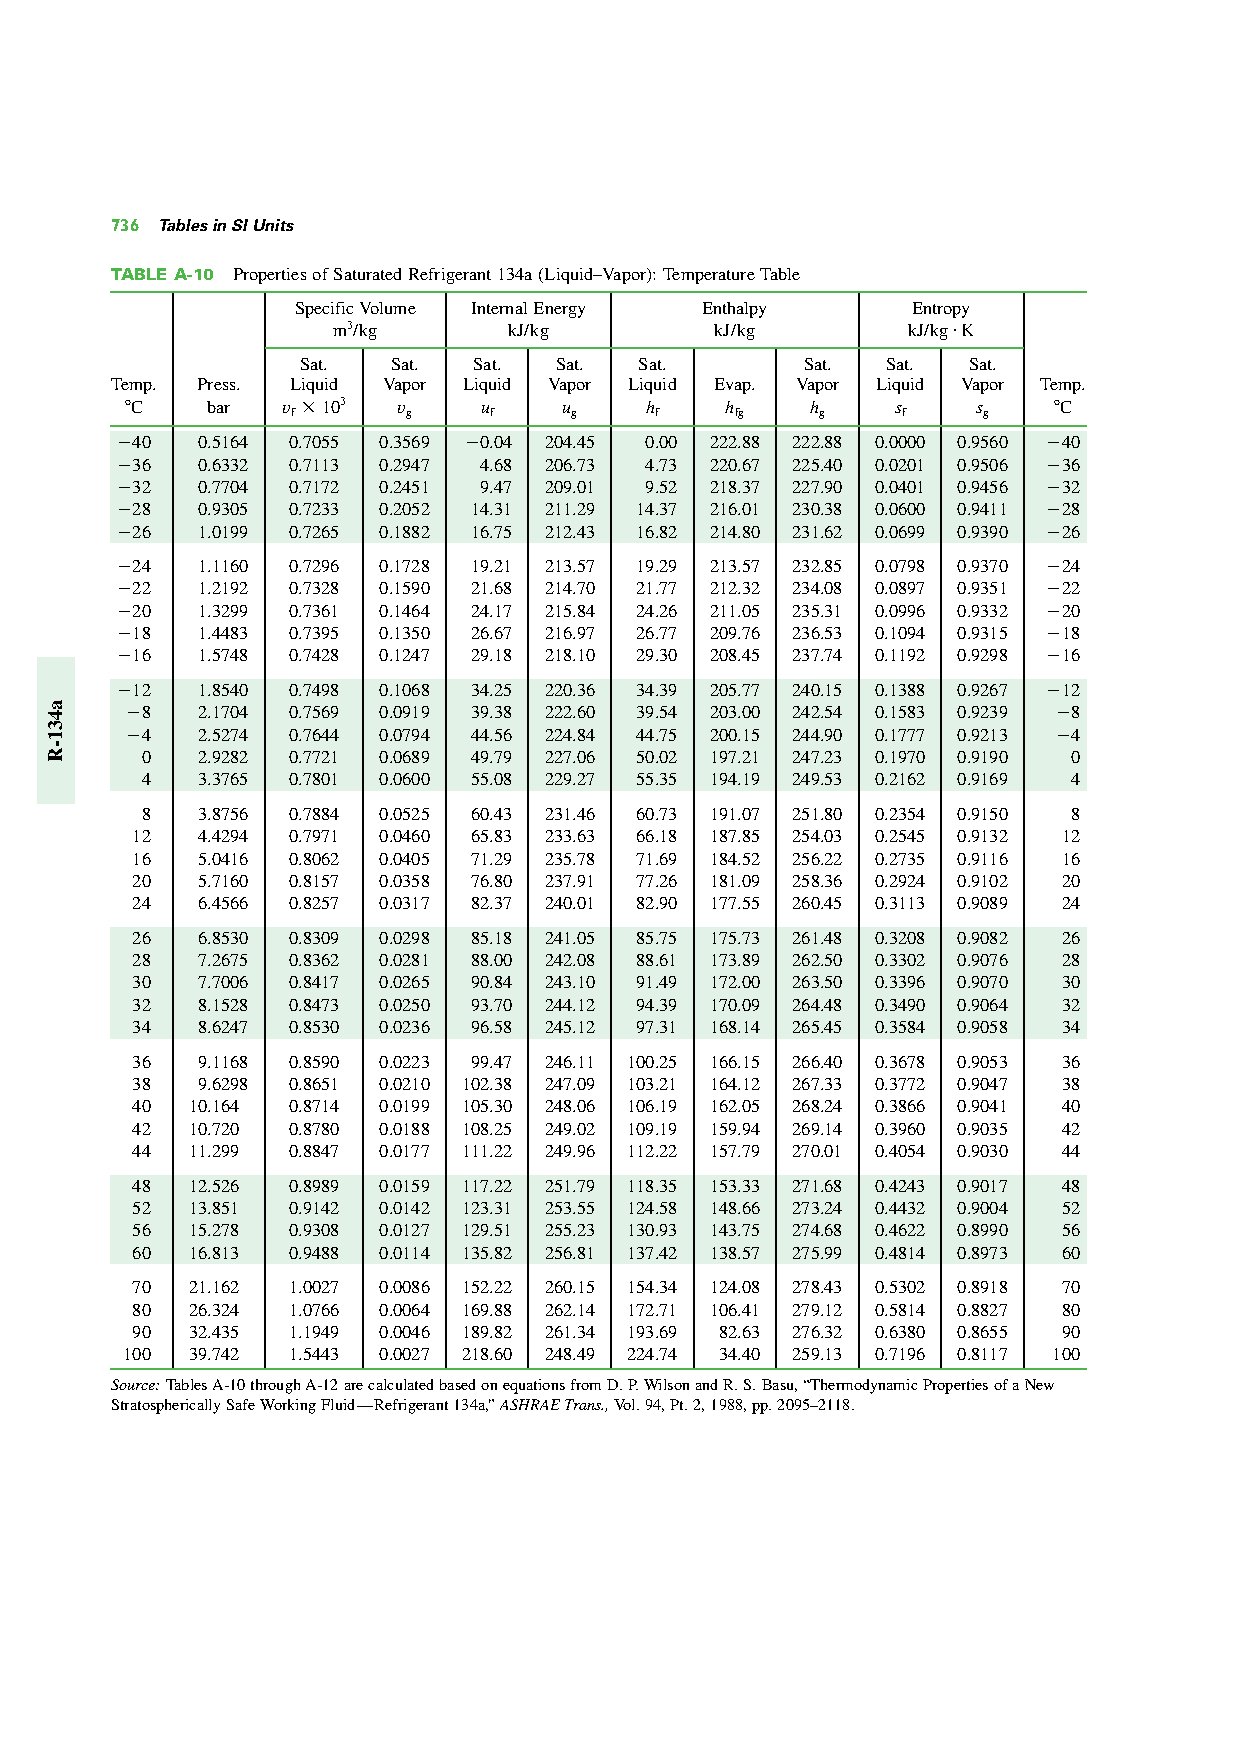
\includepdf[pages=-,fitpaper]{./Pics/Tables_R134}
}
\end{landscape}
%\end{comment}

\end{document}
